\documentclass[12pt]{report}
\usepackage{suthesis}

% -- Imports --
% (general libraries)
\usepackage[utf8]{inputenc}
\usepackage{times,latexsym,amsfonts,amssymb,amsmath,graphicx,url,bbm,rotating}
\usepackage{multirow,hhline,stmaryrd,bussproofs,mathtools,siunitx}
\usepackage{booktabs,xcolor,csquotes,calligra}
\usepackage{subcaption}

% (custom libraries)  %new
\usepackage{afterpage} %new
\usepackage{longtable} %new

% (inline references)
%\usepackage{natbib}
%\usepackage{tabularx}
\usepackage[hidelinks]{hyperref}
\hypersetup{
    colorlinks=true,
    citecolor=magenta,
    linkcolor=.,
    urlcolor=blue
}

\usepackage{epigraph}
\renewcommand{\epigraphsize}{\normalsize}
\setlength{\epigraphwidth}{0.9\textwidth}

% (tikz)
\usepackage{soul}
\definecolor{light-yellow}{RGB}{255, 255, 153}
\sethlcolor{light-yellow}

% (custom)
% (tweaks)
\definecolor{darkred}{rgb}{0.5451, 0.0, 0.0}
\definecolor{darkgreen}{rgb}{0.0, 0.3922, 0.0}

\def\blue#1{\textcolor{blue}{#1}}
\def\darkblue#1{\textcolor{blue}{#1}}
\def\red#1{\textcolor{red}{#1}}
\def\darkred#1{\textcolor{darkred}{#1}}
\def\green#1{\textcolor{green}{#1}}
\def\darkgreen#1{\textcolor{darkgreen}{#1}}
\def\yellow#1{\textcolor{yellow}{#1}}
\definecolor{burntorange}{HTML}{BF5700}
\def\orange#1{\textcolor{burntorange}{#1}}
\def\gray#1{\textcolor{gray}{#1}}
\def\darkgray#1{\textcolor{darkgray}{#1}}

\newcommand\sys[1]{\textsc{#1}}
\newcommand\longcaption[2]{\caption[#1]{#2}}

% (paper compilation hacks)
\usepackage{cite}
\definecolor{darkblue}{rgb}{0.0,0.0,0.4}


% Common hyphenations
\hyphenation{Text-Runner}
\hyphenation{Verb-Ocean}
\hyphenation{Raj-pur-kar}

%\bibliographystyle{plainnat}


% Comments
\usepackage{xspace}
\usepackage{xargs} % commandx
\setlength {\marginparwidth }{2cm}
\usepackage[colorinlistoftodos,prependcaption,textsize=tiny]{todonotes}
\usepackage{marginnote}
\usepackage{color}
\definecolor{darkgreen}{RGB}{0,100,0}

% Inline comments useful for tables and figures.
\newcommandx{\icmtl}[2][1=]{\todo[inline]{DC: #2}\xspace}
\newcommandx{\icmtm}[2][1=]{\todo[inline]{CM: #2}\xspace}

% Comments for other places.
\newcommandx{\cmtl}[2][1=]{\todo[linecolor=blue,backgroundcolor=blue!10,bordercolor=blue,#1]{DC: #2}\xspace}
\newcommandx{\cmtm}[2][1=]{\todo[linecolor=red,backgroundcolor=red!10,bordercolor=red,#1]{CM: #2}\xspace}

\newcommand\cmb[1]{\marginpar{\tiny\raggedright\textcolor{blue}{\textsf{ DC\@: #1}}}}
\newcommand\cmm[1]{\marginpar{\tiny\raggedright\textcolor{red}{\textsf{\bfseries CM\@: #1}}}}

\usepackage{enumerate}

\setcounter{secnumdepth}{3}

\usepackage{footnote}
\makesavenoteenv{tabular}
\makesavenoteenv{table}

\usepackage{xpinyin}

% -- Document --
\begin{document}

% Title
\title{PREDICTING SEA ICE IN THE ARCTIC WITH SUPERVISED LEARNING}
\author{UCL Candidate Code: KNCM2, KNHB8, NMHR0, KCSH2}
%\principaladviser{Petros Aristidou}
%\firstreader{John Green}
%\secondreader{John BigBooty}
%\thirdreader{Jane Supernumerary} %if needed
%\fourthreader{Severus Snape} %if needed



% Preface
% (notes: "...submitted..." see line 281~286 of function "titlep" in .sty )
\beforepreface
\hypersetup{linkcolor=magenta}
\prefacesection{Abstract}
Predicting future environmental information is one of the most elusive and long-standing challenges in Artificial Intelligence. This report tries to tackle the problem of predicting the Arctic sea ice: how to implement multiple Machine Learning algorithms. On the one hand, we think that Supervised Learning algorithm can predict the Arctic sea ice level. On the other hand, if we want to build an optimal predictor to ensure that our predictions on the Arctic sea ice are useful to the further future research, we would need an efficient and concise strategy to analyse the performance of different Supervised Learning algorithms. Besides, we need more strategies to analyse different factors related to the level of sea ice.

In this project, we firstly focus on Linear Regression, Penalised linear regression, Penalised Polynomial Regression, Random Forest, and Neural Networks: the most common and famous Supervised Learning algorithms by far. Then, according to the testing results, we will choose a better algorithm after testing the performance to be the algorithm that predicts the Arctic sea ice, both in a normal situation and the selected special situations.

This report consists of two parts. In the first part, we aim to understand the advantages of predicting sea ice of the Arctic and previous research on applying all kinds of algorithms on the related topic, especially predicting the Arctic sea ice or the Antarctic ice sheets. Then we present our efforts at implementing effective Supervised Learning algorithms. 

In the second part of this project, we first get our performance results with different Supervised Learning algorithms by K-fold method. This is the so-called now-forecasting. Then, based on the performance results, we predict the Arctic sea ice for the further ten years with Random Forest with different specific scenarios.
\hypersetup{linkcolor=.}
\prefacesection{Acknowledgements}
\afterpreface
\hypersetup{linkcolor=magenta}



% -- Sections --
\chapter{Introduction}                          % Chapter 1
\label{Chapter1:Intro}
% section:
\section{Motivation} %1.1

The motivation for this project includes attention to one of the most serious environmental risks on the planet in the early 21st century, the accelerating global temperature.


According to the paper from Nature, climate change happened in the past 70 years \cite{parmesan2003globally}. It has already had effects on the environment around us. Glaciers are shrinking and ices are breaking up earlier on the lakes and rivers. 

\begin{figure}[!tbh]
\center
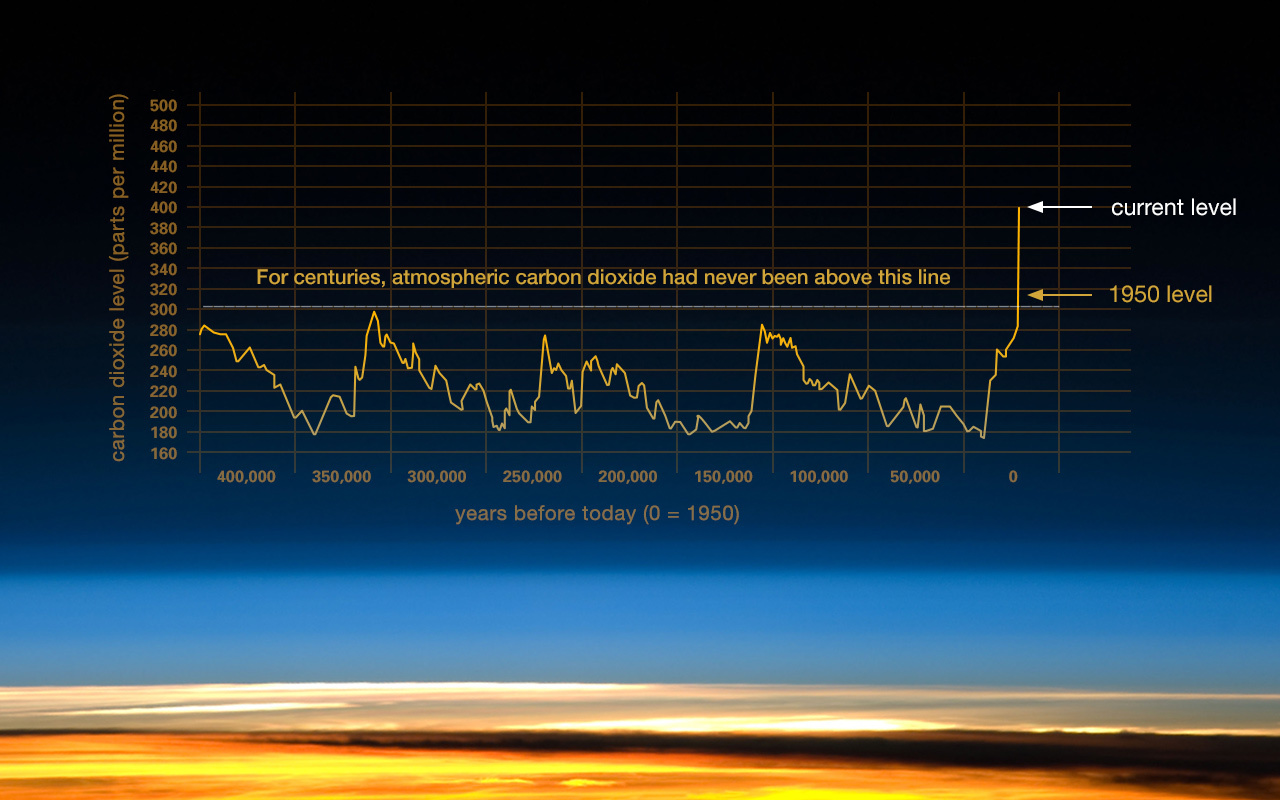
\includegraphics[scale=0.33]{Figure/1.1-NASA-CO2.jpeg}
\longcaption{The evidence that atmospheric CO2 has increased since the Industrial Revolution began}{\label{1.1-NASA-CO2} The evidence that atmospheric CO2 has increased since the Industrial Revolution began. Image courtesy: https://climate.nasa.gov/evidence}
\end{figure}

The greenhouse effect has been working since the formation of the earth. Without the greenhouse effect, the surface of the earth would be extremely cold, the temperature would drop to minus 20°C, the ocean would freeze, and life would not form. Most climate scientists agree that it is the human expansion that causes global warming \cite{epic337530}. As we know, carbon dioxide (CO2) is a significant component of the atmosphere. Atmospheric CO2 concentration has been increased by more than a third since the Industrial Revolution began \cite{epic337530}. More importantly, as shown in Figure \ref{1.1-NASA-CO2}, atmospheric carbon dioxide has exceeded the highest level in the past 400,000 years.

Therefore, what we are facing is not the issue of whether there is a greenhouse effect, but the issue that humans emit a large number of greenhouse gases into the atmosphere through the burning of fossil fuels, causing the drastic greenhouse effect and the earth’s climate.

When the world's average temperature rises by 1°C, huge changes will occur: sea levels will rise, mountain glaciers will retreat, and snow-covered areas will shrink. As the global temperature rises, it will lead to uneven precipitation. In some areas, precipitation increases, while in others, precipitation decreases. For example, the Sahel region in West Africa has been severely arid since 1965, while in North China, precipitation has been decreasing year after year since 1965. Compared with the 1950s, precipitation in North China has been reduced by 1/3, and water resources have been reduced by 1/2. China's annual drought-affected area is about 400 million acres. In normal years, the national irrigation area lacks 30 billion cubic meters of water each year, and the cities lack 6 billion cubic meters of water. 

When the average temperature of the world rises by 3°C, the world will suffer from food shortages. Due to rising temperatures, the global sea level has been rising at a rate of 1 to 2 millimetres per year in the past 100 years. It is expected that the sea level will continue to rise by 30 to 50 centimetres by 2050, which will flood a large amount of low-lying coastal land. In addition, due to climate changes have led to the aggravation of climatic disasters such as droughts, floods, and low temperatures, causing economic losses of more than tens of billions of dollars worldwide each year.


In this report, our team focuses on sea ice in the Arctic. We will look for the elements that we think affect the changes in Arctic sea ice, analyse their influence on the changes in sea ice, and select the two elements that we think are the most important. We will put these two influencing factors into our emergency model, and analyse the impact of significantly changing them on Arctic future sea ice.
\section{Report Outline} %1.2

This thesis consists of two parts --- \sys{Part I Environmental Risks in Supervised Learning: Foundations} and \sys{Part II Scenario: Predicting Arctic Sea Ice in Supervised Learning}.

\sys{Part I} focuses on the task of understanding and building Machine Learning processing flow, including processing to tidy data, so that we are able to predict Arctic sea ice in \sys{Part II}.

\begin{description}
    \item In Chapter~\ref{Chapter2:Review}, we first give an overview of the history and recent development of the field of .... Next we formally define the problem ... and its main categories. We then briefly discuss ....  Finally, we argue ....
    \item In Chapter~\ref{Chapter3:Method}, we present the ..... We begin with describing .... We then introduce ... and we describe .... 
   
\end{description}
\section{Contributions} %1.3
The contributions of this thesis are summarised as follows: 
\begin{itemize}
  \item Our team analysed seven factors influencing the sea ice and gave an result of their correlation relationships.
  
  \item Our team
  
  \item We... 
\end{itemize}

\part{Environmental Risks in Supervised Learning: Foundations}

\chapter{Literature Review}                     % Chapter 2
\label{Chapter2:Review}
% section:
% Chapter 2: Literature Review

\section{Why We Choose to Predict Sea Ice}
The change of Arctic sea ice is a sensitive indicator of climate change. The rate of Arctic sea ice disappearance exceeds even the most pessimistic climate model predictions. The current Arctic summer ice conditions are 30 years earlier than model predictions on average, and seasonal ice-free conditions are happened early \cite{stroeve_frei_mccreight_ghatak_2008}. Therefore, the prediction of sea ice is essential for understanding the future Arctic environment and global changes. Global warming has led to a reduction in sea ice and aggravated the deterioration of the Arctic environment, while the reduction in sea ice, in turn, has accelerated global warming. Increasing concentrations of greenhouse gases are playing an increasingly important role in the disappearance of the Arctic ice cap \cite{kim2019satellite}. Many studies have also linked the loss of sea ice to atmospheric circulation patterns.

\section{How to Predict Sea Ice Level Using Statistical Models}
There are many statistical models that study the relationship between the Arctic sea ice concentration and climate factors. Stroeve et al. pioneered the use of singular value decomposition SVD, empirical orthogonal function EOF and other multivariate analysis techniques, focusing on the relationship between the decline of sea ice concentration in summer and winter and the warming trend and AO driving \cite{stroeve_frei_mccreight_ghatak_2008}. TIvy et al. used the multivariate analysis technique of Code Correlation Analysis (CCA) to compare the SIC value of Hudson Bay in July from 1971 to 2005 by comparing sea surface temperature, position altitude, sea level pressure, and regional surface air temperature. Among them, in the 6-month forecast period, the forecast results are the most accurate. Surface temperature in autumn is the most influential predictor \cite{tivy2011origins}. Ahn et al. introduced the automatic regression integrated moving average (ARIMA) method for the first time into the sea ice concentration statistical model, using seven climatic factors (skin temperature, sea surface temperature, total column liquid water, total column water vapour, and instantaneous moisture flux). It is better at predicting large data sets than the single equation of the ordinary minimum hours (OLS) regression method and has higher accuracy. The average improvement of RMSE is 0.076 \cite{ahn2014statistical}. The forward stepwise regression model is used to predict summer sea ice conditions several months in advance based on four predictors which are winter multi-year combined concentration, total ice concentration in spring, North Atlantic Oscillation Index and East Atlantic Index where $\text{R}{^2}$ value is 90.7\% and $\text{MAE}$ value is 34 \cite{drobot2002practical}. In 2003, it was expanded with multiple linear regression models \cite{drobot2003long}. Finally, in 2007, on this basis, Drobot and others created a multiple linear regression model (MLR) to predict the annual minimum Arctic sea ice range for the monthly interval from February to August. The forecast data is based on the average monthly weighted index of sea ice concentration (WIC), surface skin temperature (WST), surface illuminance (WAL) and surface long-pass volume (WDL). Each MLR model is better than the climatology model \cite{drobot2006long}, but due to insufficient statistical time series modelling, the performance of machine learning models is often better than statistical models.

\section{How to Predict Sea Ice Level Using Machine Learning Models}
Machine learning models are often used to predict Arctic sea ice concentration and Arctic sea ice classification. Chi et al. used a large Arctic sea ice dataset to train a neural network to predict the Arctic sea ice concentration \cite{chi2017prediction}. The neural network prediction results that use long and short-term memory (LSTM) are better than traditional autoregressive (AR) models, and can successfully adapt to long-term data sets. The average monthly forecast error is less than 9\%, but the predictability in summer is low \cite{chi2017prediction}. Choi et al. used artificial neural networks (ANN) to make short-term predictions of the Arctic Sea Ice Concentration (SIC) \cite{choi2019artificial}. Using global SIC data for training will result in higher prediction accuracy than using only Arctic SIC data for training \cite{choi2019artificial}. Shu et al. proposed an object-based random forest (ORF) to classify the ice map types of the Arctic, and the overall classification accuracy was 90.1\%. When providing surface-related values of sea ice density and snow cover, the estimation of ice thickness can be improved \cite{shu2020discrimination}.


\section{How to Predict Sea Ice Level Using Non-Statistical Methods or Non-Machine Learning Methods}
The field of sea ice prediction is very extensive. Since 1979, the satellite-based multi-channel passive microwave imaging system has continuously monitored the Arctic sea ice concentration. Common monitoring systems are Scanning Multichannel Microwave Radiometer (SMMR), Special Sensor Microwave/Imager (SSM/I) and Advanced Microblog Scanning Radiometer (AMSR) \cite{fennig2020fundamental}. Numerical models predict interactions based on physical equations. In the short term, The prediction is usually better than the statistical model. However, it is difficult and expensive to obtain data by physical models \cite{chi2017prediction}. Sea ice retrieval algorithms usually process satellite data, and various sea ice parameters have been determined, such as age, concentration, range, thickness, etc. \cite{chi2017prediction}, but statistical models are usually better than dynamic models \cite{tivy2011origins}.


\chapter{Methodology}                           % Chapter 3
\label{Chapter3:Method}
% section:
\section{Feature Description} %3.1

The extent of Arctic sea ice in the is deemed relevant to the following nine features. The content of carbon dioxide, the area of the ozone hole over the Arctic, the land and ocean temperature in the northern hemisphere, the Max/Ave/Min temperature of North Slope Alaska, the rainfall in the Arctic, daylight of Arctic and the population of the world.

\begin{figure}[htbp]
\center
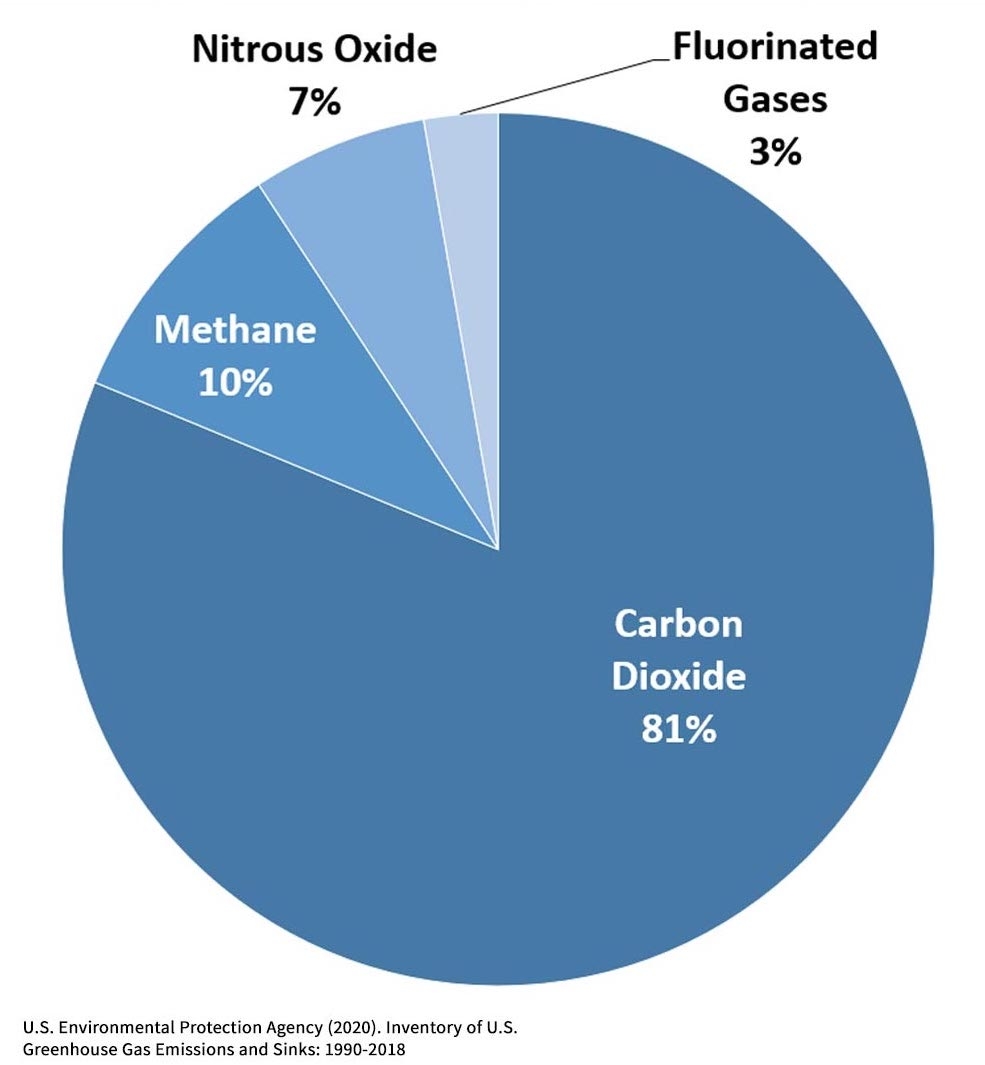
\includegraphics[width = 0.55\textwidth]{Figure/3.1-GreenHouseGas.jpg}
\longcaption{Overview of US Greenhouse Gases in 2018}{\label{3.1-GreenHouseGas} Overview of US Greenhouse Gases in 2018.\\ Image courtesy: https://www.epa.gov/ghgemissions/overview-greenhouse-gases}
\end{figure}

Changes in the area of sea ice in the Arctic are believed to be related to the content of carbon dioxide. As shown in Figure \ref{3.1-GreenHouseGas}, Carbon dioxide accounts for 81\% of greenhouse gases. Thus the main component of greenhouse gases is carbon dioxide, which is also the main cause of the greenhouse effect. According to J.H.Mercer, the greenhouse effect will have a catastrophic impact on the ice sheets \cite{mercer1978west}. Thus the content of carbon dioxide is chosen to be one of the features.

In addition, according to the results of the common correlated effects mean group (CCEMG) estimator, the GDP growth and the population size influence CO2 emission levels positively and significantly, at both the global and regional levels \cite{DONG2018180}. In that case, the GDP growth and the population size would have an impact on the ice sheets.

The ozone hole area is also considered to be related to the area of sea ice in the Arctic. In 2010, Sigmond and Fyfe found that the ozone depletion leads to a positive SAM response in austral summer, which induces sea ice melt \cite{sigmond2010has}. In that case, changes in the size of the ozone hole would also affect the changes in sea ice area. Thus the ozone hole area is chosen to be one of the features.

Furthermore, the temperature is deemed to be related to the area of sea ice in the Arctic. According to Ditlevsen and Grinsted's research, by considering a minimal model of an ice sheet, it shows that fluctuating temperatures have an effect on the mass balance and thus on the steady-state volume of the ice sheet \cite{mikkelsen2018influence}. Thus the temperature is considered to be a feature. In our project, we initially selected five different temperatures related to the Arctic area which are the ocean temperature in the Northern Hemisphere, the land temperature in the Northern Hemisphere, the maximum temperature of North Slope Alaska, the average temperature of North Slope Alaska, and the minimum temperature of North Slope Alaska.

Changes in the area of sea ice in the Arctic are also believed to be related to the rainfall. According to Bromwich and Robasky, the increased precipitation may reduce the net loss of ice sheets area or even turn it into net gain \cite{Bromwich1993RecentPT}. Thus rainfall is considered to be a feature.


The amount of daylight in the Arctic is also believed to be related to the area of ice sheets. The Arctic has polar day and polar night phenomena, so there is periodicity in the phenomenon of daylight. As shown in Figure \ref{3.1-daylight}, due to the sunshine could produce heat, thus different amount of daylight time would affect the temperature. Thus the daylight is considered to be a feature.


\begin{figure}[htbp]
\center
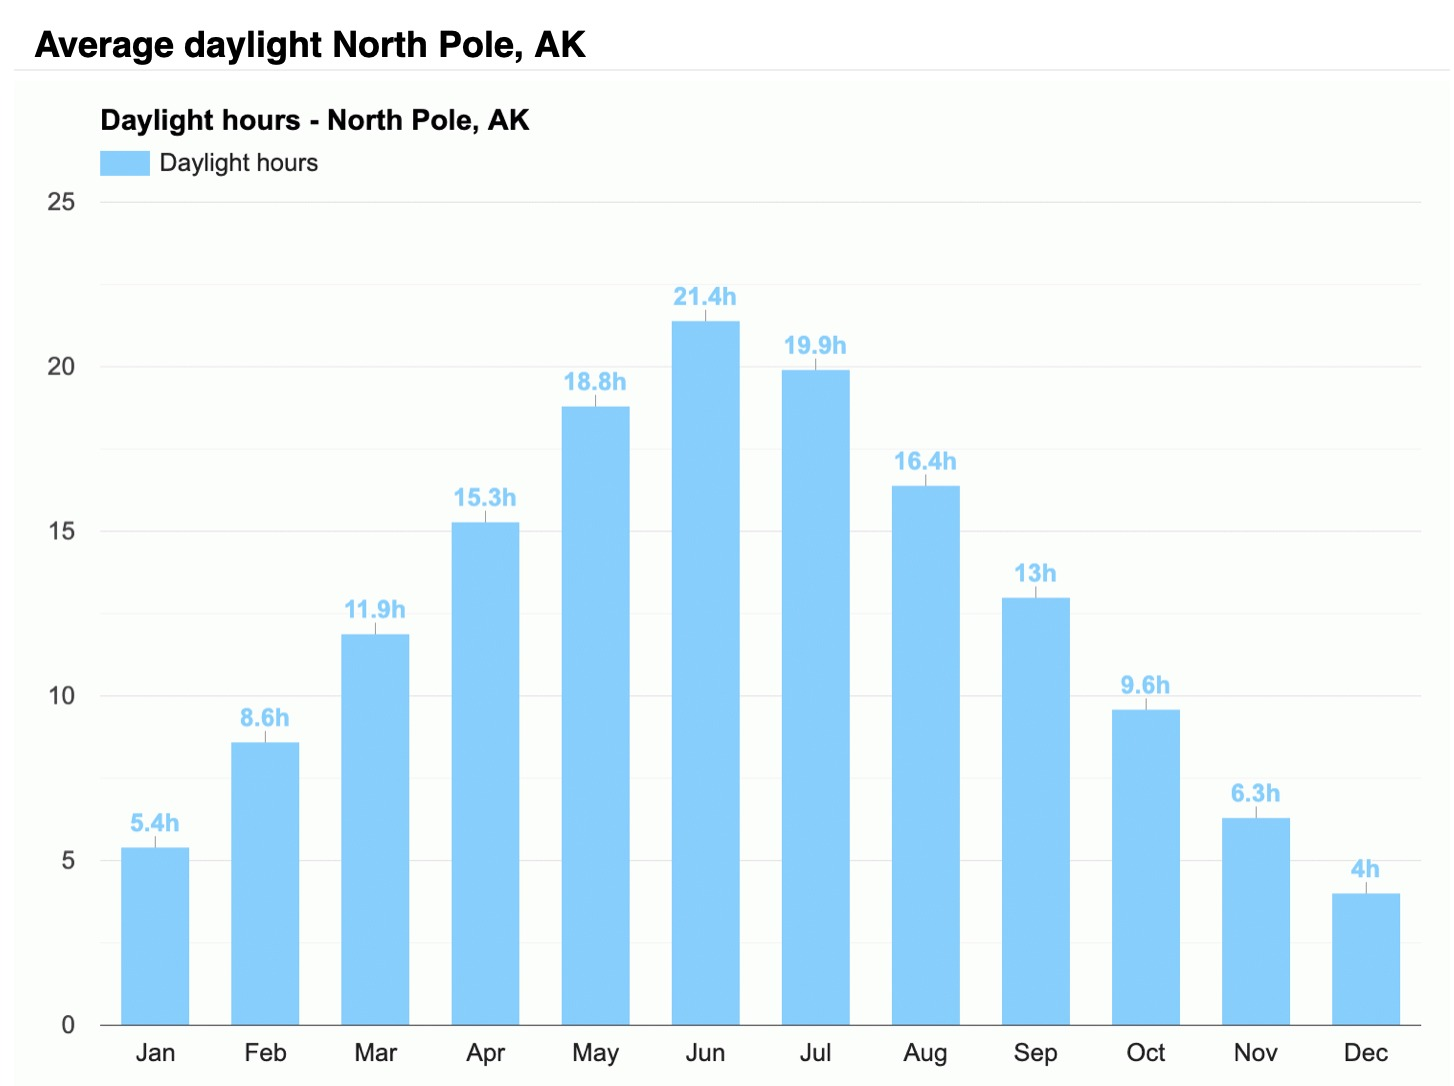
\includegraphics[width = 0.7\textwidth]{Figure/3.1-daylight.jpeg}
\longcaption{Average daylight in North Pole, Alaska}{\label{3.1-daylight} Average daylight in North Pole, Alaska. Image courtesy: https://www.weather-us.com/en/alaska-usa/north-pole-climate}
\end{figure}

\section{Data} %3.2
For Y-axis, data for Arctic sea ice could be found in National Snow \& Ice Data Centre (NSIDC). For X-axis, data for global CO2 content and Arctic ozone hole area are made available to public via the National Aeronautics and Space Administration (NASA) website. Data for global population were accessed through the Our World in Data website. In addition, data for the different temperatures and rainfall and average daylight of Arctic are provided by National Oceanic and Atmospheric Administration (NOAA) and Weather Atlas website respectively. Furthermore, the data for the global GDP could be found in the world bank website.

All X-axis data are selected from January 1980 to October 2020 and been divided by month. When collecting the data, some data is divided according to the year as a unit, so it is necessary to convert these data into a month as the unit to divide. For example, for the data of population, first subtract the total population in 1980 from the total population in 1979, and then divide the difference into 12 equal parts, and evenly distribute them to each month in 1980, so as to get the 12 months’ data of population in 1980. However, some data sets may lack partial months of data. Thus, first look for data at the same month of other years, and then use the method of means of regression to calculate the missing data.

In order to meet the standard of normalisation, the first data of the set should be 0, which means each data should be subtracted from the value of the first data. Furthermore, all data should be divided by the value of the last data, thus all data would be controlled between 0 and 1, which is convenient for adjusting parameters in subsequent analysis.


%\begin{figure}[!t] % t means top
%    \center
%    \includegraphics[scale=0.5]{img/google_search.pdf}
%    \caption{.....}
%\end{figure}
\section{Model Accuracy} %3.4

\subsection{Mean Squared Error}
Mean Squared Error (MSE) is generally used to observe the deviation between the predicted and true value of the model. MSE (Function \ref{eq:MSE}) is used to measure the accuracy between testing results from models. MSE is the expectation of the sum of squared residuals between the true value and predicted value. The smaller the MSE value, the better the performance of the model in the testing process.
\begin{eqnarray}
    {\text{MSE} ={\frac {1}{N}}\sum _{n=1}^{N}(y_{n}-{\hat {y_{n}}})^{2}}
    \label{eq:MSE}
\end{eqnarray}


\subsection{R-squared}
R-squared ($\text{R}^{2}$) (Function \ref{eq:R-squared}) is the sum of squares of residuals over the total sum of squares, where the value lies between 0 and 1. It is used to compare the performance of the training results from each training data set. The greater the $\text{R}^{2}$, the better the performance of the model in the training process.

\begin{eqnarray}
    \text{R}^{2} = {1}-{\frac {\text{SS}_{\text{residual}}}{\text{SS}_{\text{total}}}}
    \label{eq:R-squared}
\end{eqnarray}
\section{Now Forecasting Methodology} %3.5

\subsection{K-Fold Cross-validation}
\begin{figure}[htbp]
    \center
    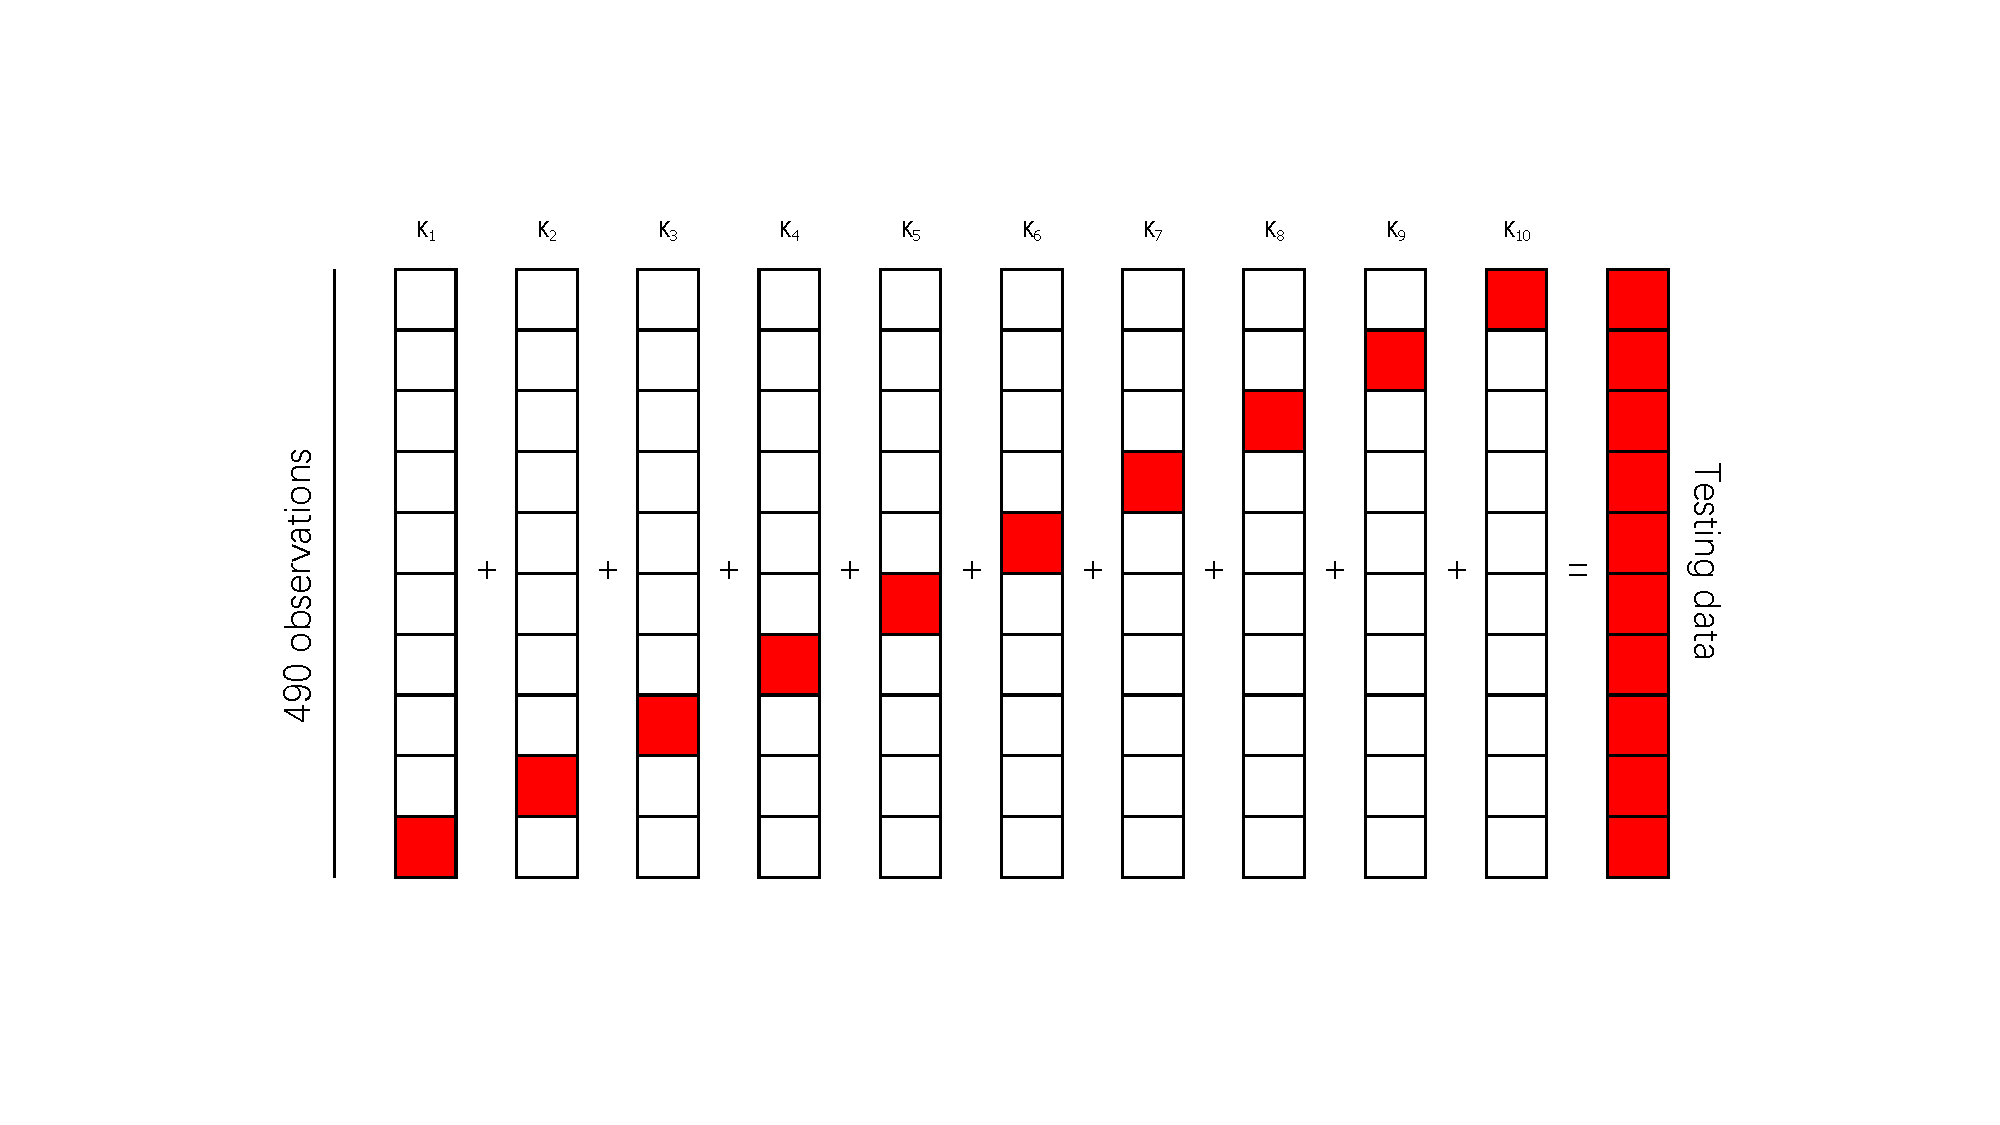
\includegraphics[scale=0.4]{Figure/3.5.1-K-Fold.pdf}
    \caption{K-fold Cross-validation}
    \label{3.5.1-K-Fold}
\end{figure}

Cross-validation is a data splitting and testing method. In this project, k-fold splits the data set into 10 parts. Each time, 9 parts represented by the white grid in Figure \ref{3.5.1-K-Fold} are used as training data, and the remaining part represented by the red grid in Figure \ref{3.5.1-K-Fold} is used as testing data for model validation. Since k-fold cross-validation is suitable for small data scenarios, it was applied in this project where only 490 observations are contained in the data set.


\subsection{Linear Regression}
Linear regression uses statistical analysis to determine the quantitative relationships between multiple variables \cite{montgomery2012introduction}. By a given training set, one reasonable method to pick or learn the parameters $\theta$ is to make the hypothesis $h(x)$ close to $y$. To formalize this, we will define a function that measures, for each value of the $\theta$'s, how close the $h (x^{(i)})$'s are to the corresponding $y^{(i)}$'s. We define the cost function or ordinary least squares:

\begin{eqnarray}
    J_\theta = \frac{1}{2} \sum_{i=1}^{n}{(h_\theta (x^{(i)}) - y^{(i)})^2}.
    \label{eq:cf}
\end{eqnarray}

After minimising the sum of the residual, the weights vector for each independent variable will be generated. In the result, P-value of each feature is also notable and can be applied to express the magnitude of the significant influence of the independent variable on the dependent variable. However, owing to the low deviation of linear regression, as the number of features increases, it is susceptible to high variance or over-fitting.

\subsection{Penalised Linear Regression (Lasso, min/1se)}
Comparing with linear regression, Penalised regression is a highly computationally efficient prediction method that can reduce a large number of features into a manageable set and make good predictions on various large data sets, especially when the features are correlated.\cite{bowles2015machine}. As Function \ref{eq:new-cf} shown, a penalty term with coefficient Lambda is added to cost function to penalise model complexity by limiting the weight magnitude for reducing the variance.

\begin{eqnarray}
    J_\theta := J_\theta + \lambda \sum_{K=1}^{k}{b_k}.
    \label{eq:new-cf}
\end{eqnarray}

In the project, Lasso regression was applied. Comparing with ridge regression, which is also a form of Penalised Regression, Lasso regression is able to cancel unimportant features based on the choice of Lambda. Generally, the choice of Lambda is based on the MSE. In this algorithm, the k-fold method was applied for calculating MSE with a different value of Lambda. 

Based on MSE, there are two methods to choose coefficient Lambda which are \sys{min} and \sys{1se}. These two methods have different preferences. Applying \sys{min} is intended to obtain the model with the minimum error and the most accurate, while \sys{1se} tends to simplify the model as much as possible with the loss of a small amount of accuracy.

\subsection{Penalised Polynomial Regression (Lasso, min/1se)}
For linear regression and penalised linear regression, due to the lack of flexibility, the fitting result is often poor. Facing this problem, features with higher-order were applied in them for training. Similarly, when the features of higher-order were added to the model for raising flexibility, the polynomial regression may also have the problem of over-fitting. Therefore, similar to linear regression, Lasso penalisation was also added, simplifying models while addressing the problem of over-fitting.

\subsection{Random Forest}
Random Forest is a model that uses the main vote of multiple decision trees to achieve prediction. It can be applied both on regression and classification algorithm \cite{tan2018prediction}. For Random Forest, $n$ training samples with $i$ features (less than the total number of features) are randomly selected from the original data sets using Bootstrapping method that is a type of reaping sampling method. After $k$ rounds of random selection, $k$ independent training sets are selected and $k$ decision trees are generated.

Due to the randomness of observation selection, non-selected observations are defined as out-of-bag data. Use these observations as labelled testing data, out-of-bag errors (\sys{OOB}) can be calculated. As  $k$ increases, \sys{OOB} will decrease and tend to be stable. Selecting the appropriate k value based on the \sys{OOB} is critical.  Small $k$ value causes \sys{OBB} instability  while great $k$ value brings high Computational cost.

Also, the feature number applied in each decision tree $i$ can be also important. Small $i$ value causes low flexibility problem, while great $i$ value reduce the diversity of the "forest". Generally, with the increase of $i$, \sys{OOB} value drops first and then rises. Choosing the $i$ value corresponding to the minimum \sys{OBB} helps to achieve better performance of the model.

\subsection{Neural Networks}
A neural network is a massively parallel processor composed of simple processing units. Neurons are formed the basic structure of the network. With the structure of multiple hidden layers, Neural networks algorithm is highly flexible for fitting but also suffers from over-fitting and high computational cost problem. 

Forward propagation is a process that multiple inputs enter a hidden layer and time corresponding weights. After that, a nonlinear activation function is applied to convert the input signal into an output signal. For training Neural Networks, backpropagation method is applied. Through gradient descent of loss function, the weights in the whole network can be updated. Since the application of differential operation, the computational cost of training can be mainly attributed to backpropagation.







\section{Future Forecasting Methodology} %3.6
\subsection{Normal Situation} %3.6.1
\label{sec:normal-predic}
In order to predict the Arctic sea ice extent variation in the next 10 years, the existing features will be processed in three ways to obtain the value of each feature from the year of 2021 to 2030.
\begin{enumerate}[(a)]
    \item 
        \textbf{Pure Periodical Feature (Daylight, Rainfall)}. Theses features are monthly-average values over years since 20th century. They would be applied on the predictions for the next 10 years.
        
    \item
        \textbf{Data with Accessible Future Scenario (Population, GDP, CO2)}. Since the future variation scenarios are given, the monthly record in scenarios would be applied directly.
    \item
        \textbf{Other data (Ozone, Temperature related features)}. As no future variation scenario was found, the values of future 10 years would be generated by applying existing trends via linear regression.
\end{enumerate}

The way of generating future data is based entirely on recent trends, so the predicted result would be treated as \sys{Normal Situation}. It would be compared as criteria against forecast based on \sys{Special Situations} which would be discussed in the following part.


\subsection{Special Situation} %3.6.2
The \sys{Special Situations} was defined as the prediction of the Arctic sea ice variation under the circumstance that the fluctuation of a feature does not follow the trend of previous years. Firstly, two feature that has the most significant impact on extent variation would be obtained by variable importance analysis as key factors. For the key factors, two different scenarios would be generated, correspondingly representing sharper and smoother variation comparing with \sys{Normal Situation}.


\part{Scenario: Predicting Arctic Sea Ice in Supervised Learning}


\chapter{Now Forecasting Results}   % Chapter 4
\label{Chapter4:Now-Results}
% section:
\section{Correlation matrix} %4.1

\begin{figure}[htbp]
\centering
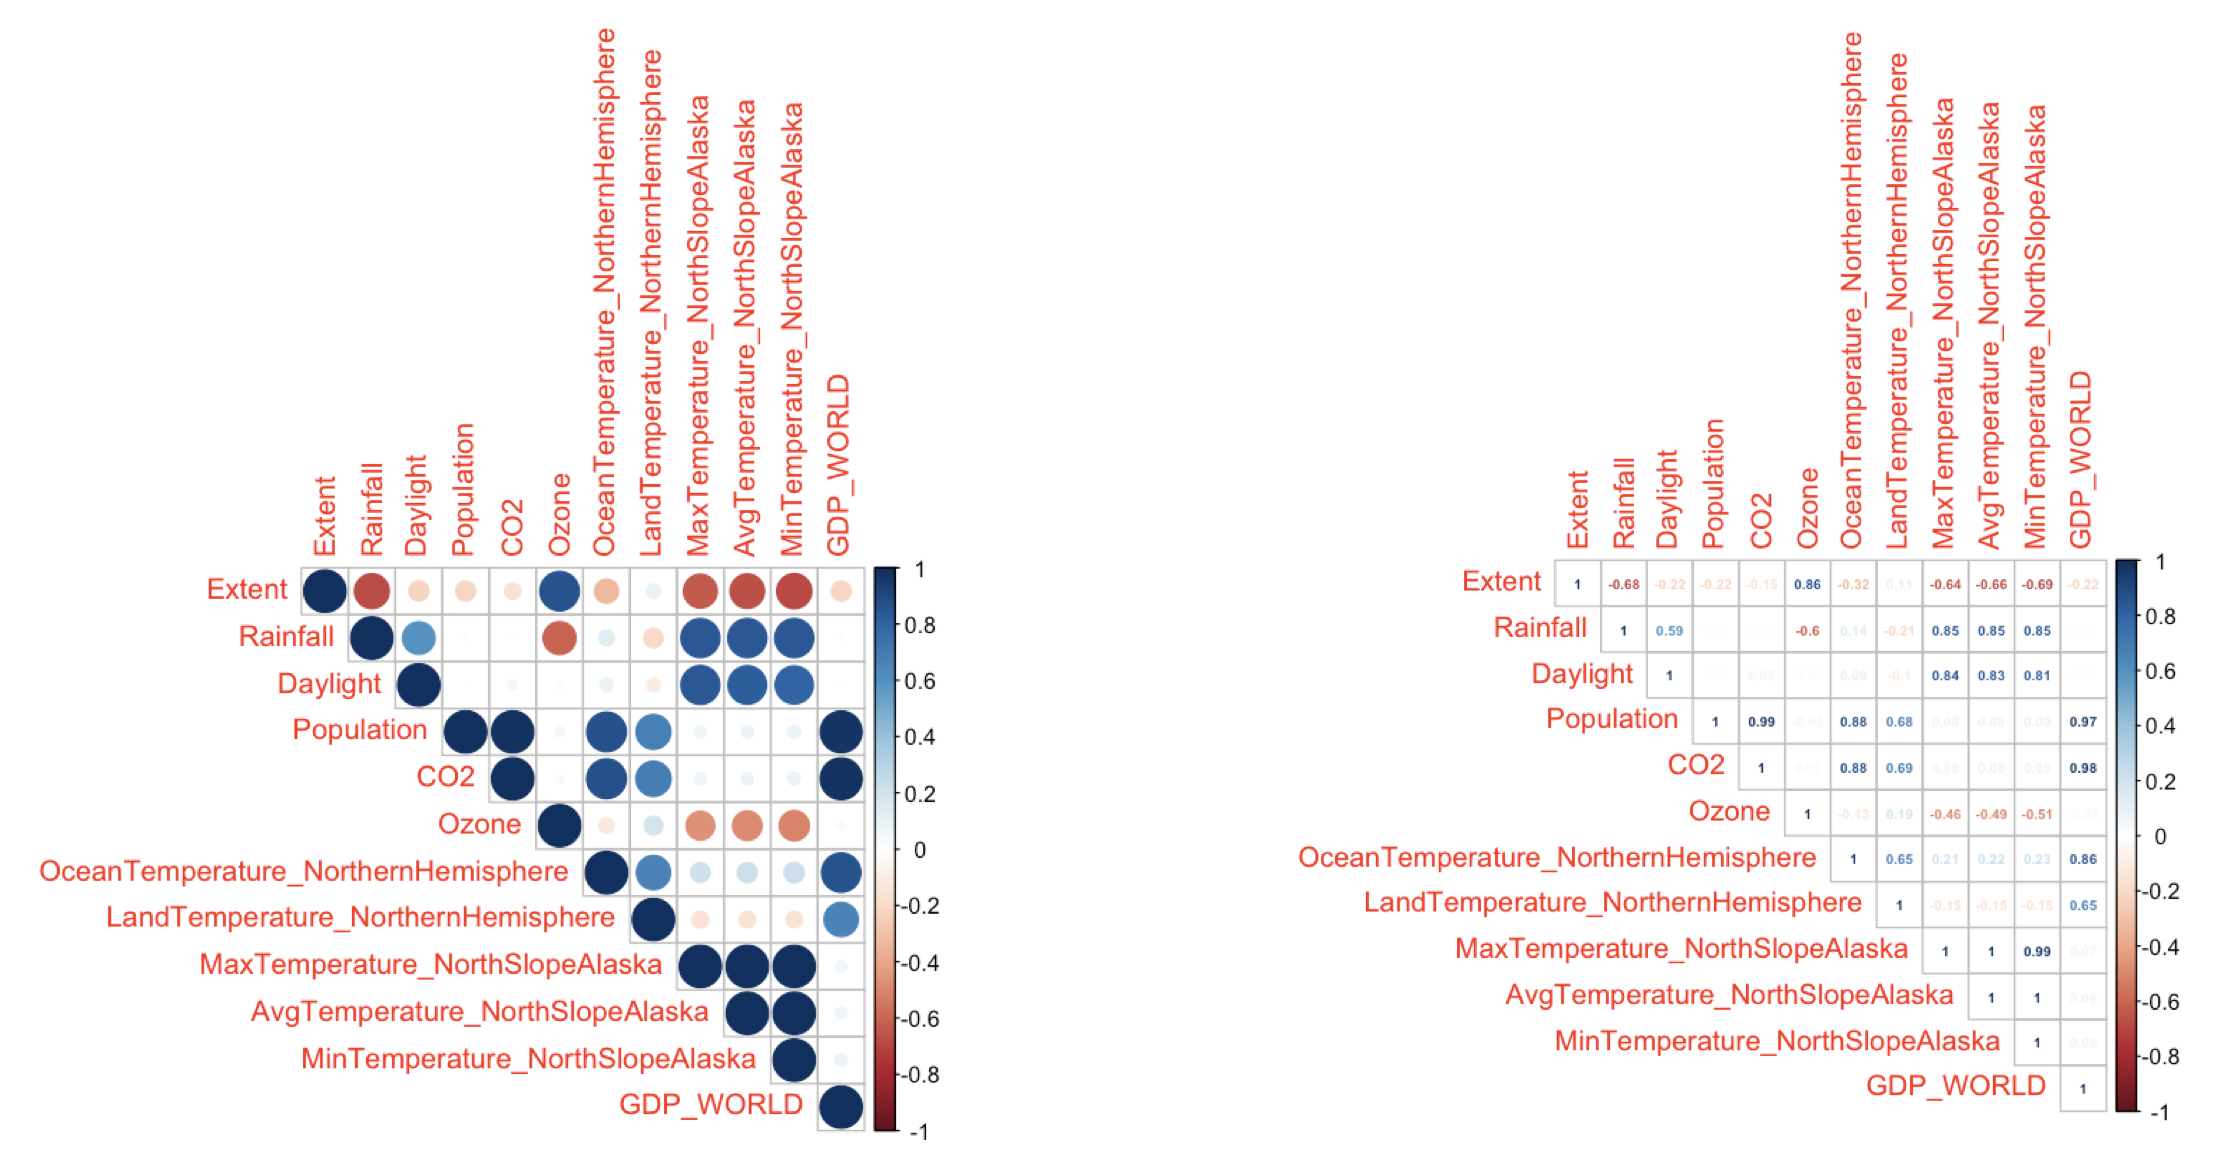
\includegraphics[width = 1.0\textwidth]{Figure/4.1-CM.png}
\caption{Left: The correlation matrix with "circle" method. Right: The correlation matrix with "number" method.}
\label{4.1-CM}
\end{figure}
The correlation matrix is a symmetric matrix. Based on the results of the Correlation Matrix, it shows that the extent of Arctic sea ice has a strong correlation with ozone, temperature gained from North Slope Alaska, and rainfall. The temperature measured in the North Pole Alaska is divided into maximum, average, and minimum temperatures. These three measured temperature values are not only highly correlated with extent but also highly correlated with each other. Therefore, it is unreasonable to add all three variables into the model. Here, the feature with the greatest correlation (min temperature) was selected by Correlation Matrix through number but not through symbol. Hence, the minimum temperature gained from North Slope Alaska was selected.
\section{Linear Regression} %4.2

In the first algorithm, Linear Regression model provides a basic fitting results. Without the addition of penalty term, $\text{R}^2$ reached 0.8982 (as Figure \ref{4.2.1-LR-Training-Results} shown), the mean square error (MSE) reached 0.00946 when the test set was used for evaluation.

\begin{table}[htbp]
  \centering
  \footnotesize
  \begin{tabular}{p{5.75cm} | c c c c c c}
  \toprule
  Coefficients: \\ %row 1
    & Estimate & Std. Error & t value & $\text{Pr}(>|\text{t}|)$\\
  \hline
  (Intercept) & 0.72626 & 0.02602 & 27.912 & $< \text{2e-16}$ & ***\\
  Rainfall & 0.04478 & 0.02495 & 1.799 & 0.0727 & .\\
  Daylight & 0.18852 & 0.03376 & 5.583 & $\text{3.95e-08}$ & ***\\
  Population & -0.98423 & 0.13192 & -7.461 & $\text{4.07e-13}$ & ***\\
  CO2 & 1.86621 & 0.19379 & 9.630 & $< \text{2e-16}$ & ***\\
  Ozone & 0.39157 & 0.03262 & 12.003 & $< \text{2e-16}$ & ***\\
  OceanTemperature\_NorthernHemisphere & -0.23312 & 0.04408 & -5.289 & $< \text{1.87e-07}$ & ***\\
  LandTemperature\_NorthernHemisphere & 0.08561 & 0.03910 & 2.190 & 0.0290 & *\\
  MinTemperature\_NorthSlopeAlaska & -0.63691 & 0.05038 & -12.642 & $< \text{2e-16}$ & ***\\
  GDP\_WORLD & -69403 & 0.07102 & -9.772 & $< \text{2e-16}$ & ***\\
  \hline
  \multicolumn{6}{l}{Signif. codes: 0 '***' 0.001 '**' 0.01 '*' 0.05 '.' 0.1 '' 1} \\
  \multicolumn{6}{l}{Residual standard error: 0.08382 on 480 degrees of freedom}\\
  \multicolumn{6}{l}{   15894 observations deleted due to missingness}\\
  \multicolumn{6}{l}{Multiple R-squared: 0.8982,      Adjusted R-squared: 0.8963}\\
  \multicolumn{6}{l}{F-statistic: 470.5 on 9 and 480 DF, P-value: $< \text{2e-16}$}\\
  \bottomrule
  \end{tabular}
  \caption{Linear Regression training results.}
  \label{4.2.1-LR-Training-Results}
\end{table}


\begin{figure}[htbp]
\centering
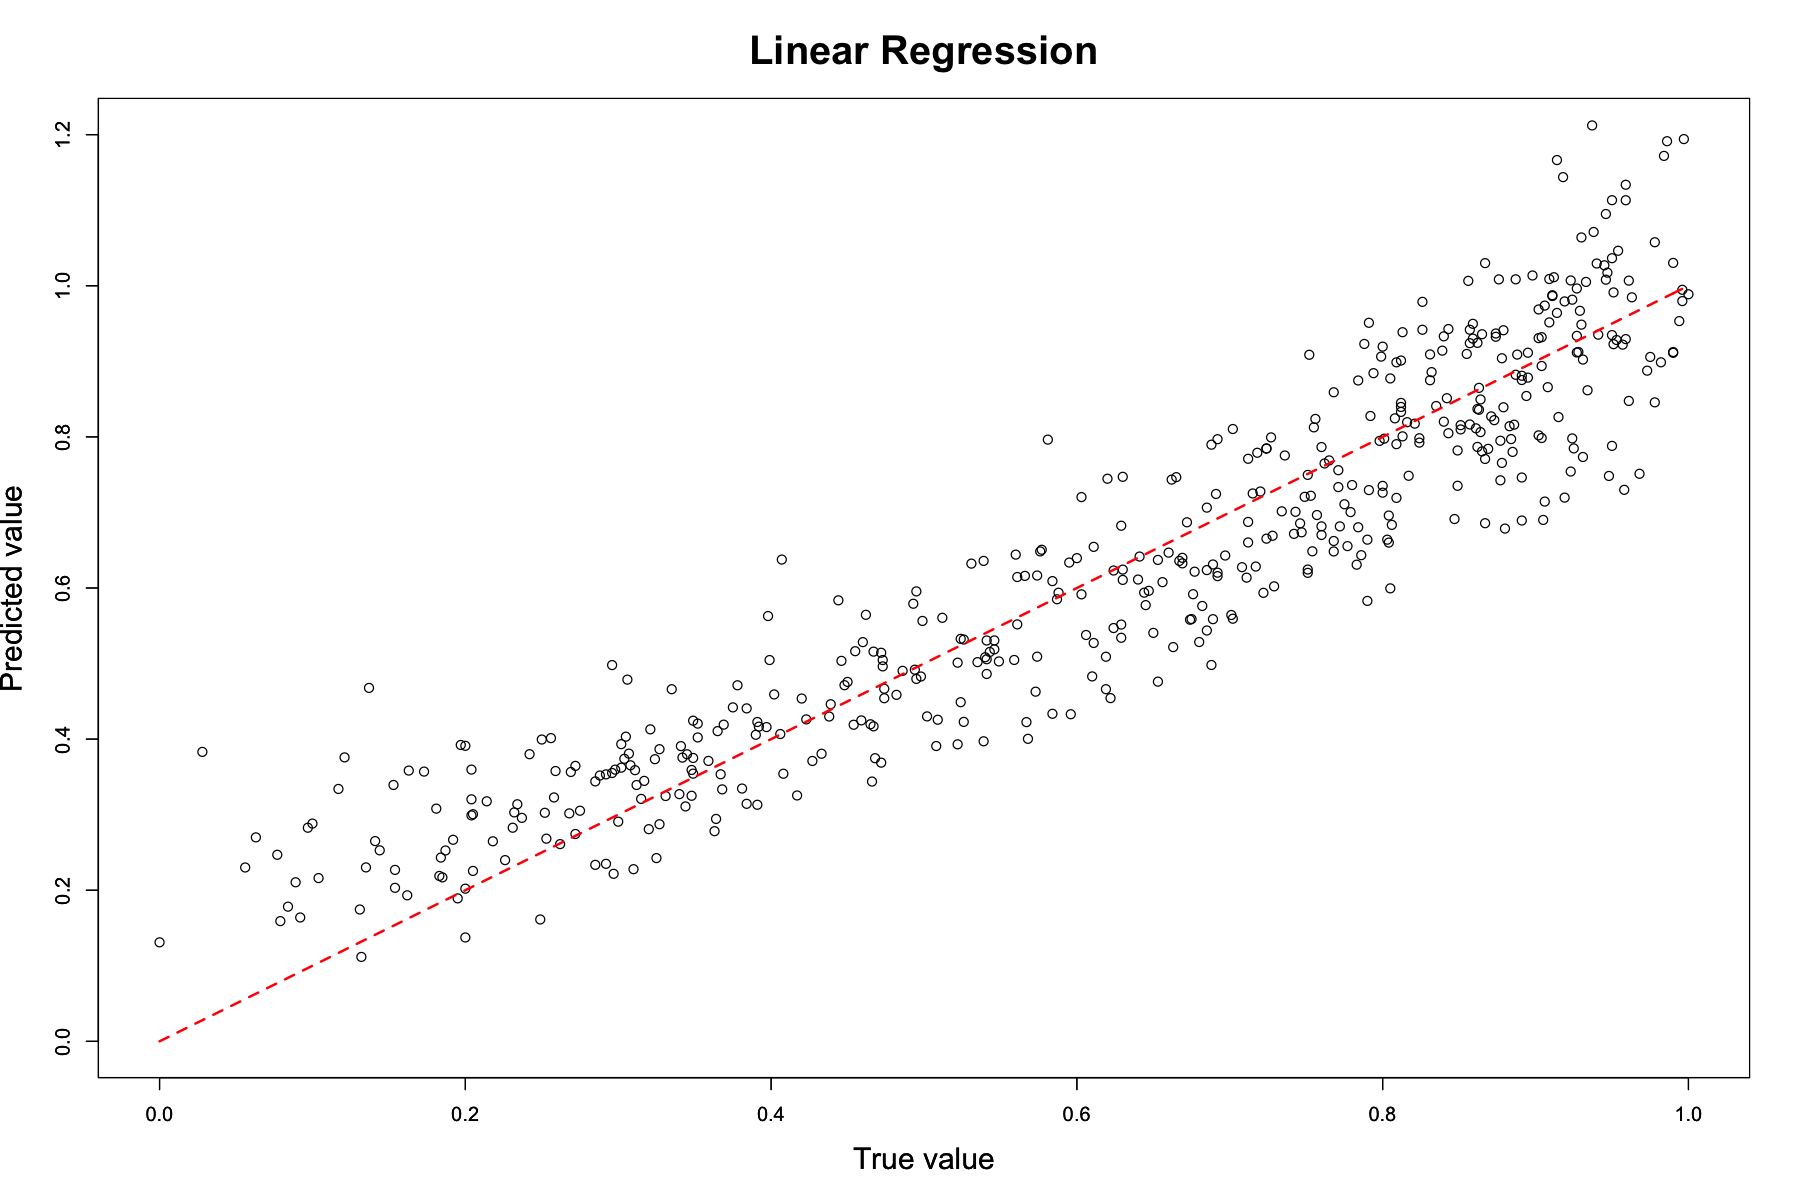
\includegraphics[width = 1.0\textwidth]{Figure/4.2.1-LR.png}
\caption{The predicted Arctic sea ice extent value vs the real Arctic sea ice extent value with \textbf{Linear Regression}. The red referenced dotted line represents the straight line y=x. Mean Square Error (MSE) is \textbf{0.00946}.}
\label{4.2.1-LR}
\end{figure}

Fitting diagram was generated as Figure \ref{4.2.1-LR}. It shows that the fitting points are not concentrated around the straight line $y=x$. In fact, this prediction was over-fitting. Comparing to other models that will be discussed later, the MSE of Linear Regression is relatively bigger, which means Linear Regression cannot predict the sea ice very well.

\newpage
\section{Penalised Linear Regression (Lasso, min/1se)} %4.3

In order to simplify the model by reducing the number of features whilst increasing the accuracy, Lasso Penalisation was applied. Using the \sys{glmnet} package, the weights of all features were presented as the change of Lambda value.

The ridge-trance figure (Figure \ref{4.2.2-NEW-PLR-ridge-trance-Log-Lambda}) shows that more and more coefficients become zero as the value of log lambda increases. In Lasso Penalisation, the features with poor performance are removed to reduce the complexity of the model.


\begin{figure}[htbp]
\center
  \begin{subfigure}{7.5cm}
    \centering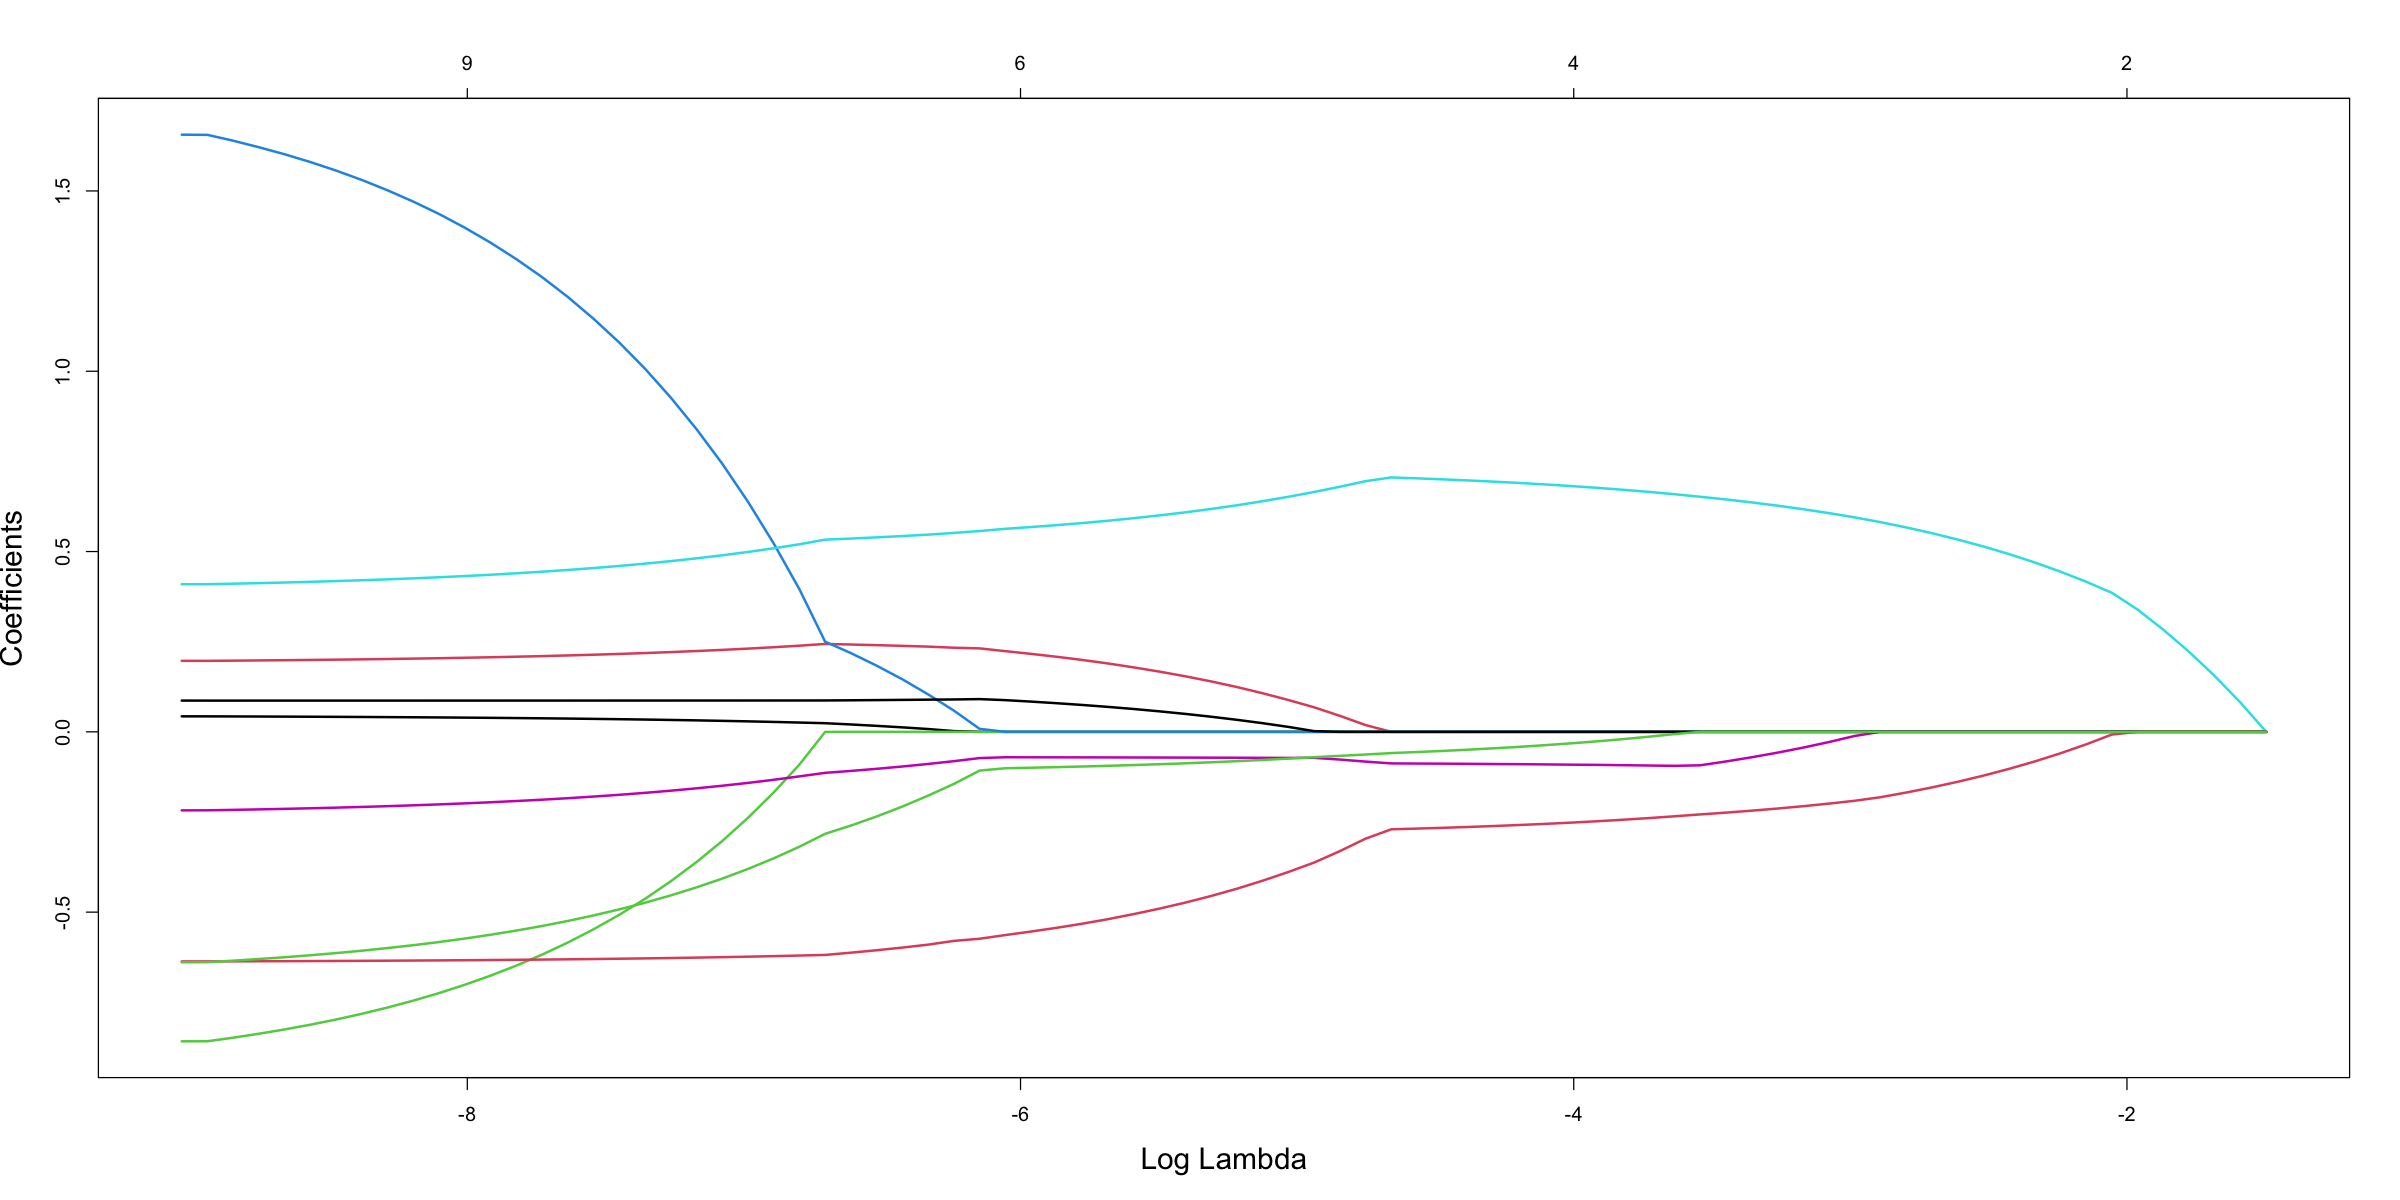
\includegraphics[width=7cm]{Figure/4.2.2-PLR-ridge-trance.png}
  \end{subfigure}
  \begin{subfigure}{7.5cm}
    \centering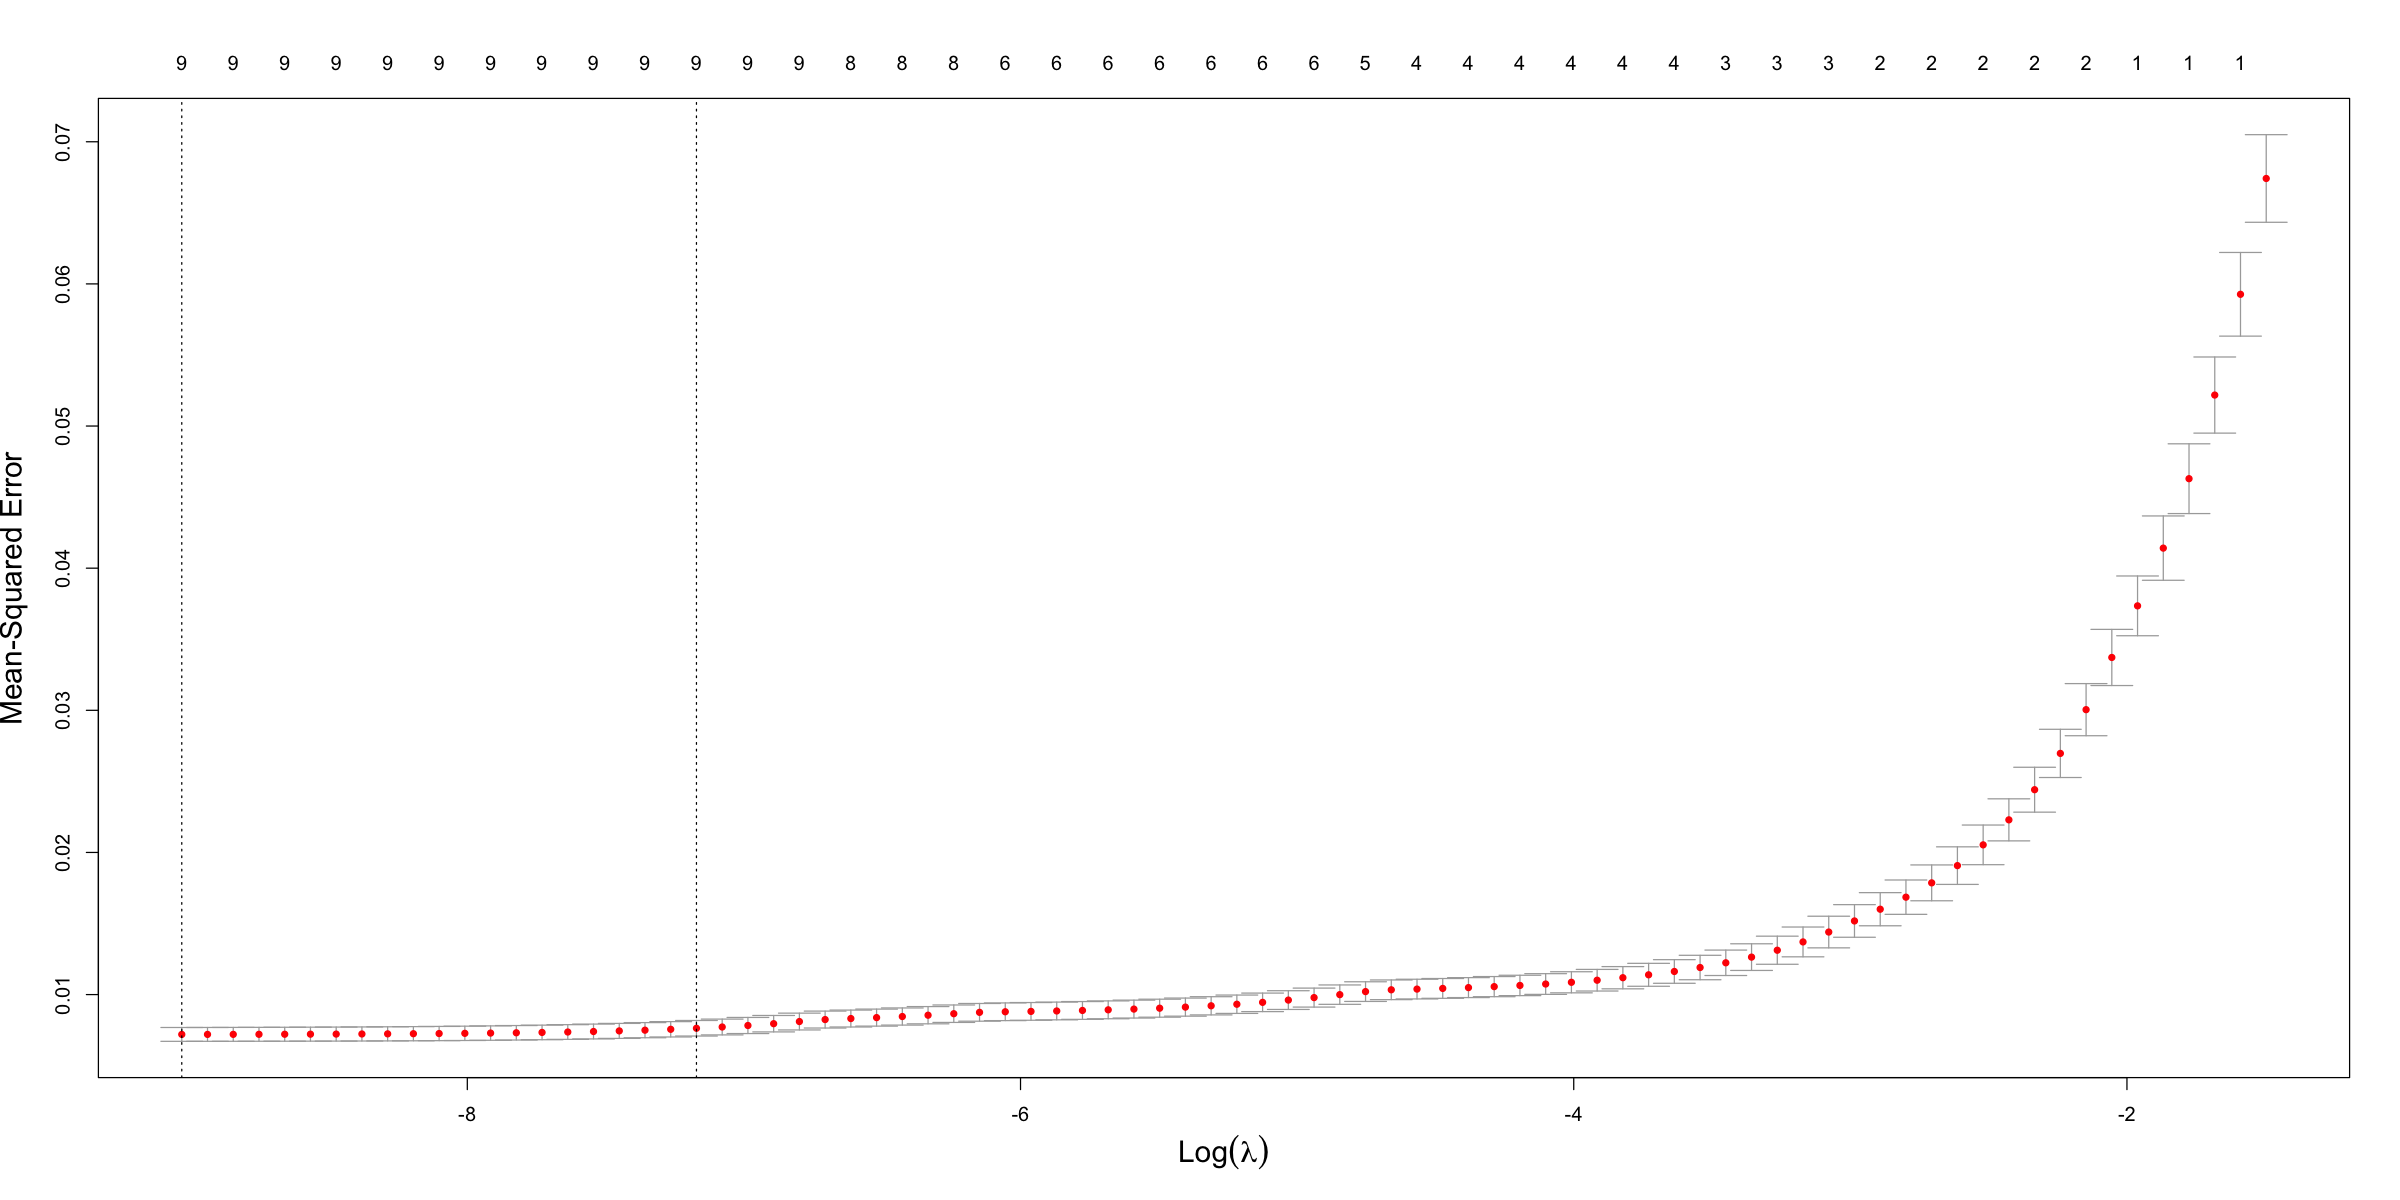
\includegraphics[width=7cm]{Figure/4.2.2-PLR-Log-Lambda-vs-Testing-Error.png}
  \end{subfigure}
  \caption{Left: Ridge trace diagram of Penalised Linear Regression. Right: Log Lambda vs Testing Error diagram of Penalised Linear Regression.}
  \label{4.2.2-NEW-PLR-ridge-trance-Log-Lambda}
\end{figure}


At this point, appropriate Lambda values were selected to output the weights of all features. In the selection, \sys{min} and \sys{1se} were applied respectively (Figure \ref{4.2.2-NEW-PLR-ridge-trance-Log-Lambda}).


Applying different options for the Lambda value, two different sets of results were obtained. When Lambda option was \sys{min}, the MSE value of the model was 0.00690, which was slightly less than the 0.00734 when Lambda option was \sys{1se}. 

The output result was demonstrated in Table \ref{4.2.2-PLR-para}. In this case, using \sys{1se} did not reduce the complexity of the model but the number of features. Therefore, \sys{min} was better than \sys{1se} in Lasso Penalisation in our project.

\begin{table}[htbp]
  \centering
  \footnotesize
  \begin{tabular}{p{5.75cm} | c | c}
  \toprule
  Coefficients: & min & 1se\\ %row 1
  \hline
    & 1 & 1\\
  (Intercept) & 0.71559335 & 0.66666336\\
  Rainfall & 0.04299020 & 0.03049067\\
  Daylight & 0.19686230 & 0.22725958\\
  Population & -0.85828586 & -0.30290499\\
  CO2 & 1.65605218 & 0.74378027\\
  Ozone & 0.40941811 & 0.48953790\\
  OceanTemperature\_NorthernHemisphere & -0.21778615 & -0.14950798\\
  LandTemperature\_NorthernHemisphere & 0.08669526 & 0.08684475\\
  MinTemperature\_NorthSlopeAlaska & -0.63667606 & -0.62486026\\
  GDP\_WORLD & -0.63894945 & -0.40706240\\
  \bottomrule
  \end{tabular}
  \caption{Hyper-parameters of Penalised Linear Regression.}
  \label{4.2.2-PLR-para}
\end{table}


In Linear Regression, the performance of test fitting was not ideal even it was optimised because of the lack of flexibility of the model. By adding a penalty term to the Linear Regression, the performance of test fitting was improved by both \sys{Min} and \sys{1SE} options. 


\begin{figure}[htbp]
\center
  \begin{subfigure}{7.5cm}
    \centering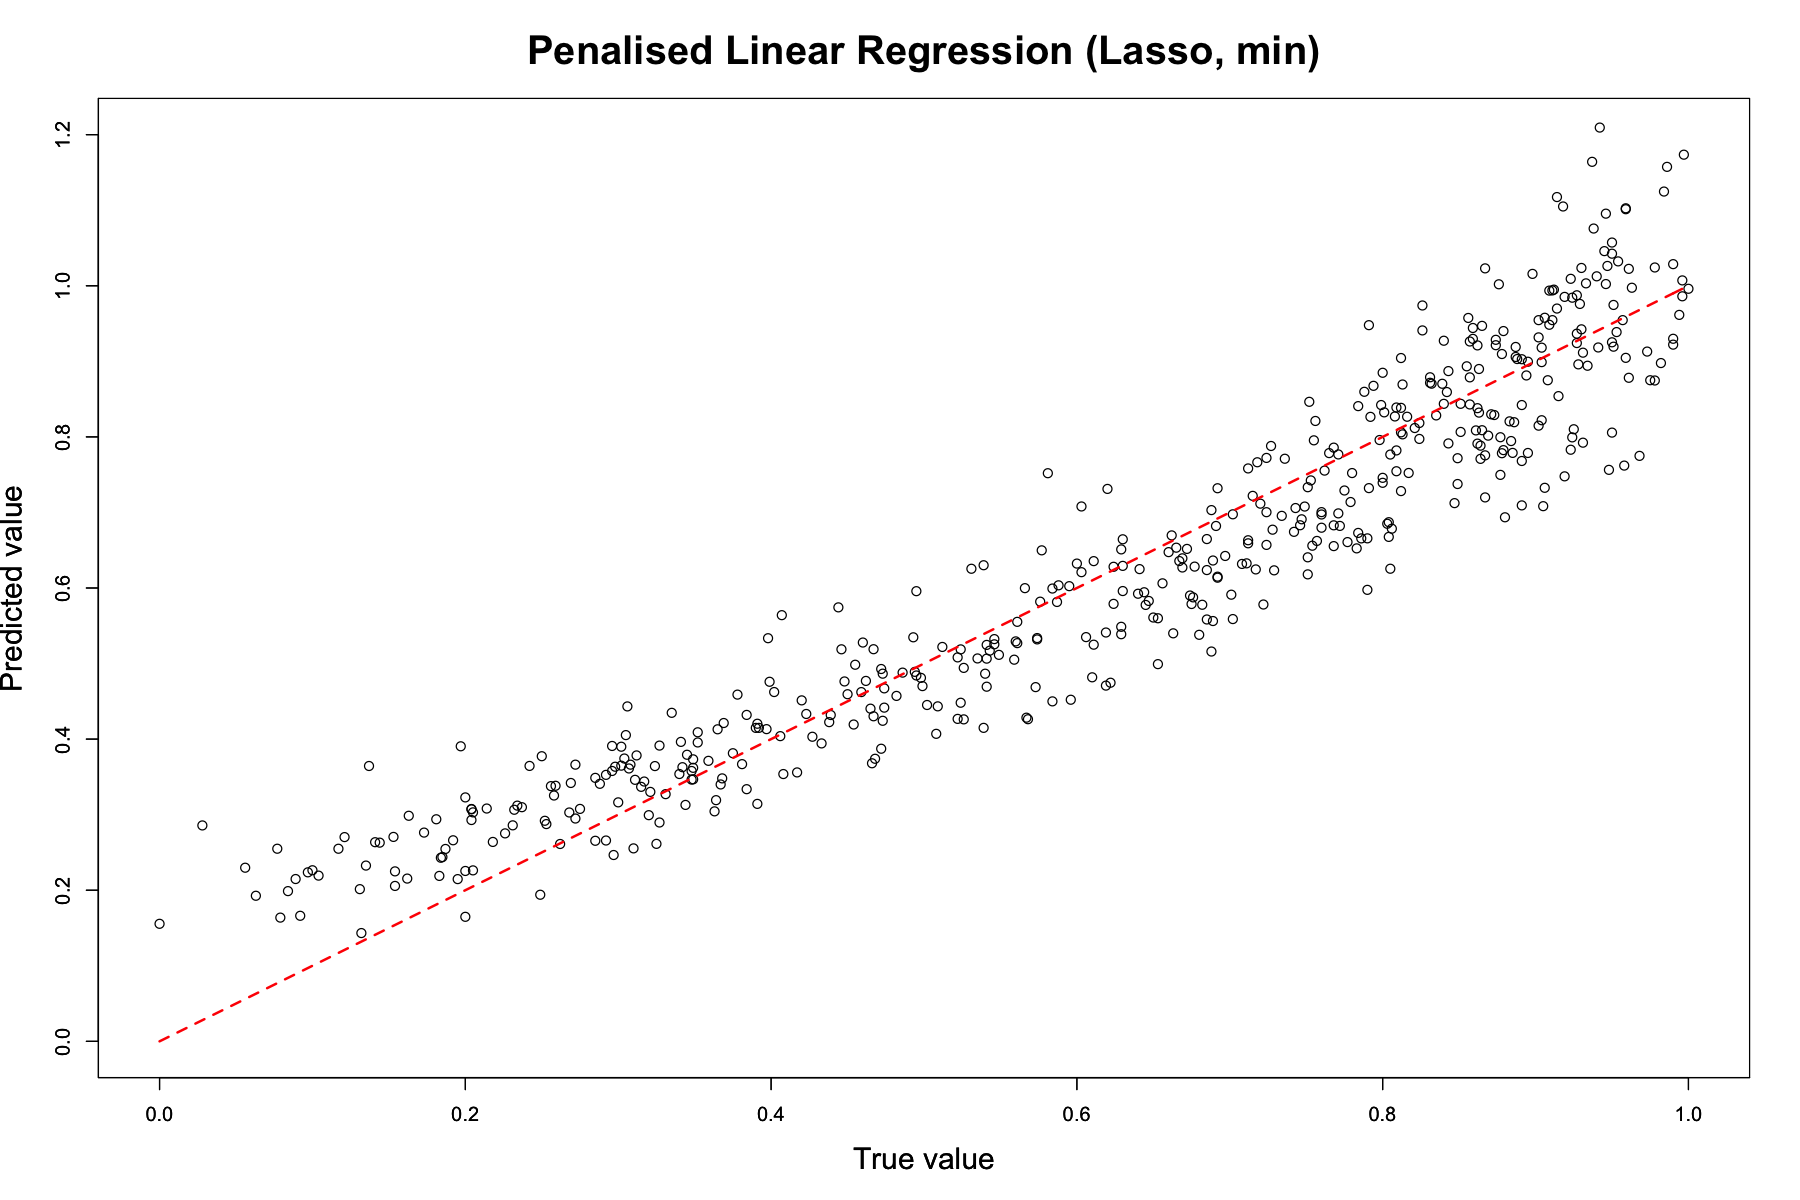
\includegraphics[width=7cm]{Figure/4.2.2-PLR-min.png}
  \end{subfigure}
  \begin{subfigure}{7.5cm}
    \centering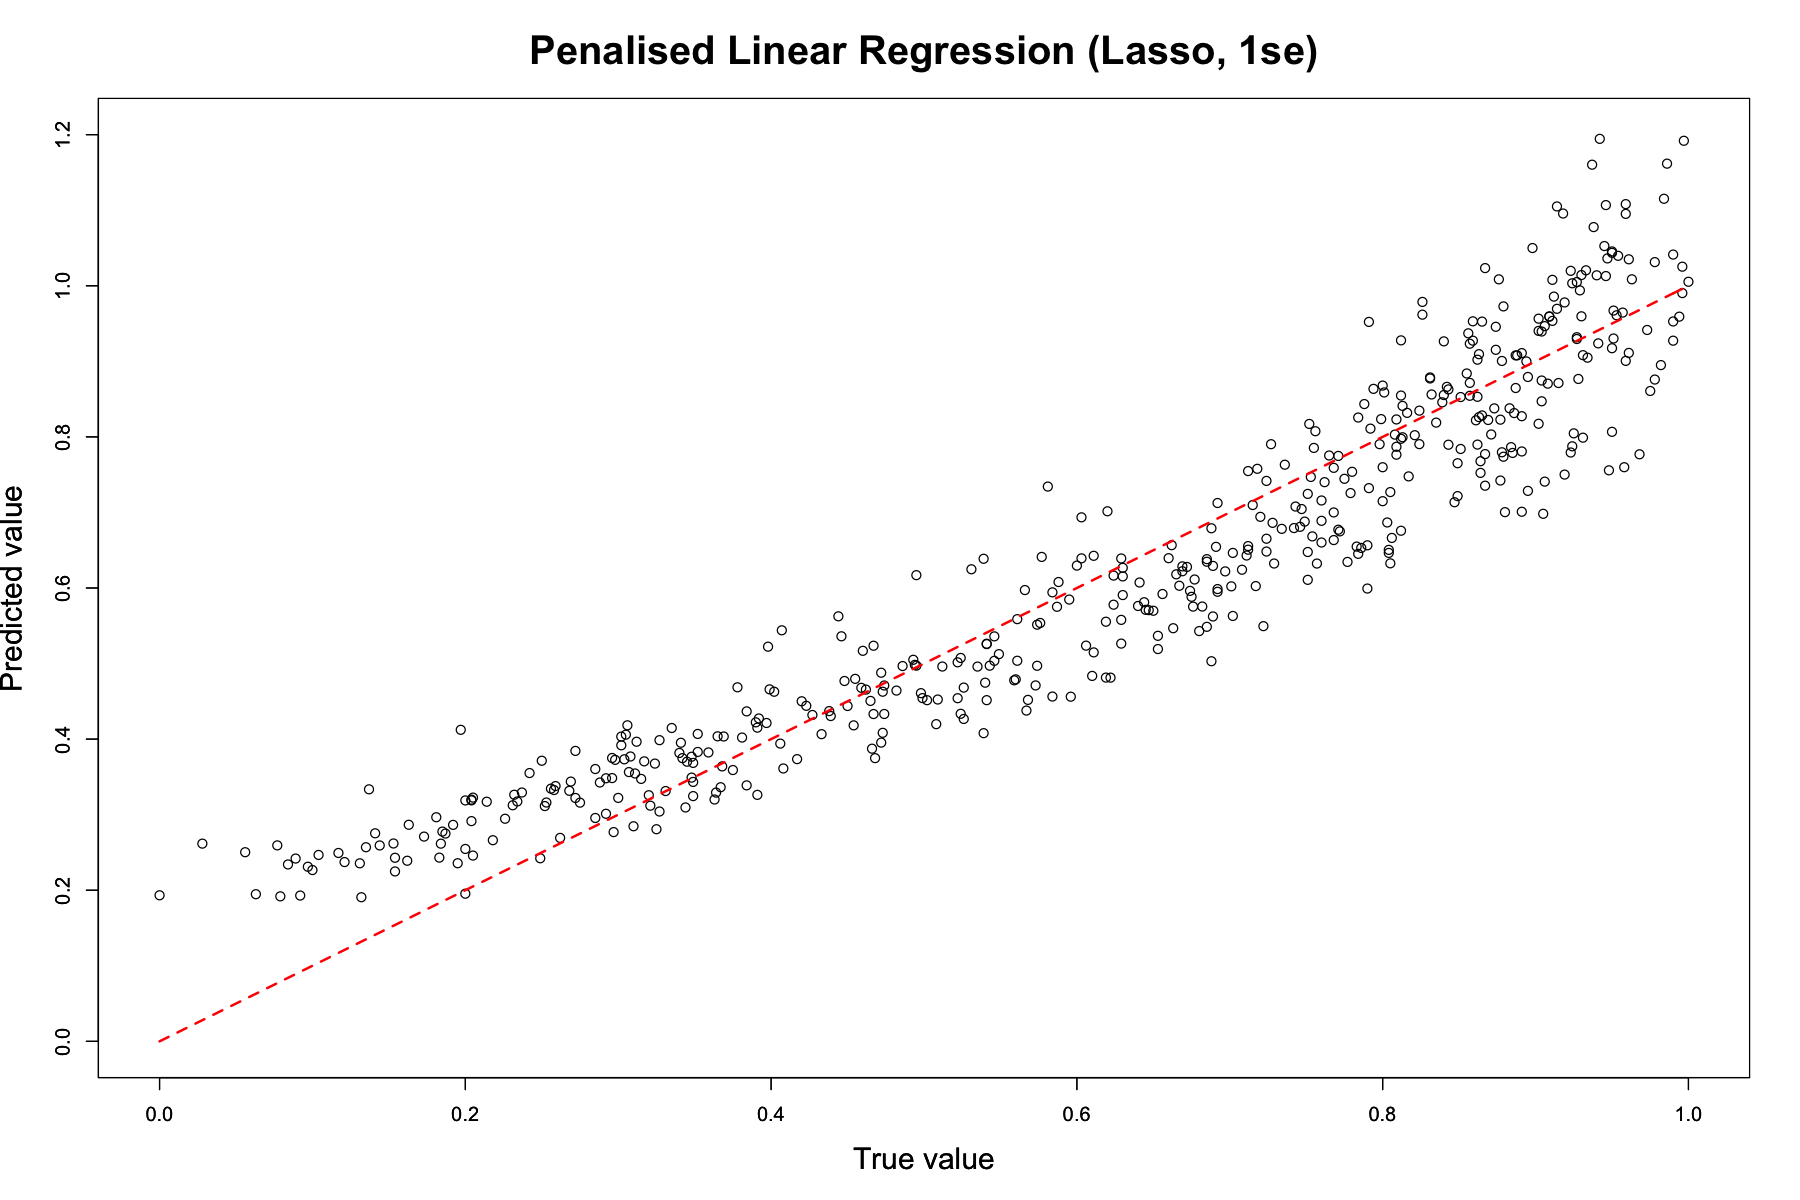
\includegraphics[width=7cm]{Figure/4.2.2-PLR-1se.png}
  \end{subfigure}
  \caption{\textbf{Left}: The predicted Arctic sea ice extent value vs the real Arctic sea ice extent value with \textbf{Penalised Linear Regression} (Lasso, \textbf{min}). The red referenced dotted line represents the straight line y=x. Mean Square Error (MSE) is \textbf{0.00690}. \textbf{Right}: The predicted Arctic sea ice extent value vs the real Arctic sea ice extent value with \textbf{Penalised Linear Regression} (Lasso, \textbf{1se}). The red referenced dotted line represents the straight line y=x. Mean Square Error (MSE) is \textbf{0.00732}.}
  \label{4.2.2-PLR-min-1se}
\end{figure}

\newpage
\input{Chapters/Chapter4-Now-Results/4-Penalised-Polynomial-Regression }
\section{Random Forest} %4.5

To use Random Forest, three parameters had to be determined which are the number of total features, the number of trees, and the number of features that randomly applied in each tree (\sys{mtry}). 

Firstly, nine out of eleven features were applied on this algorithm based on correlation matrix. Then, the "tree number vs out-of-bag error" graph (the right of Figure \ref{4.2.6-RF-200Trees-5Features}) was plotted. Based on different \sys{mtry} values, when the tree number approaches 200, the out-of-bag error tends to be stable. Hence, 200 was chosen as the tree number of this model.


\begin{figure}[htbp]
\center
  \begin{subfigure}{7.5cm}
    \centering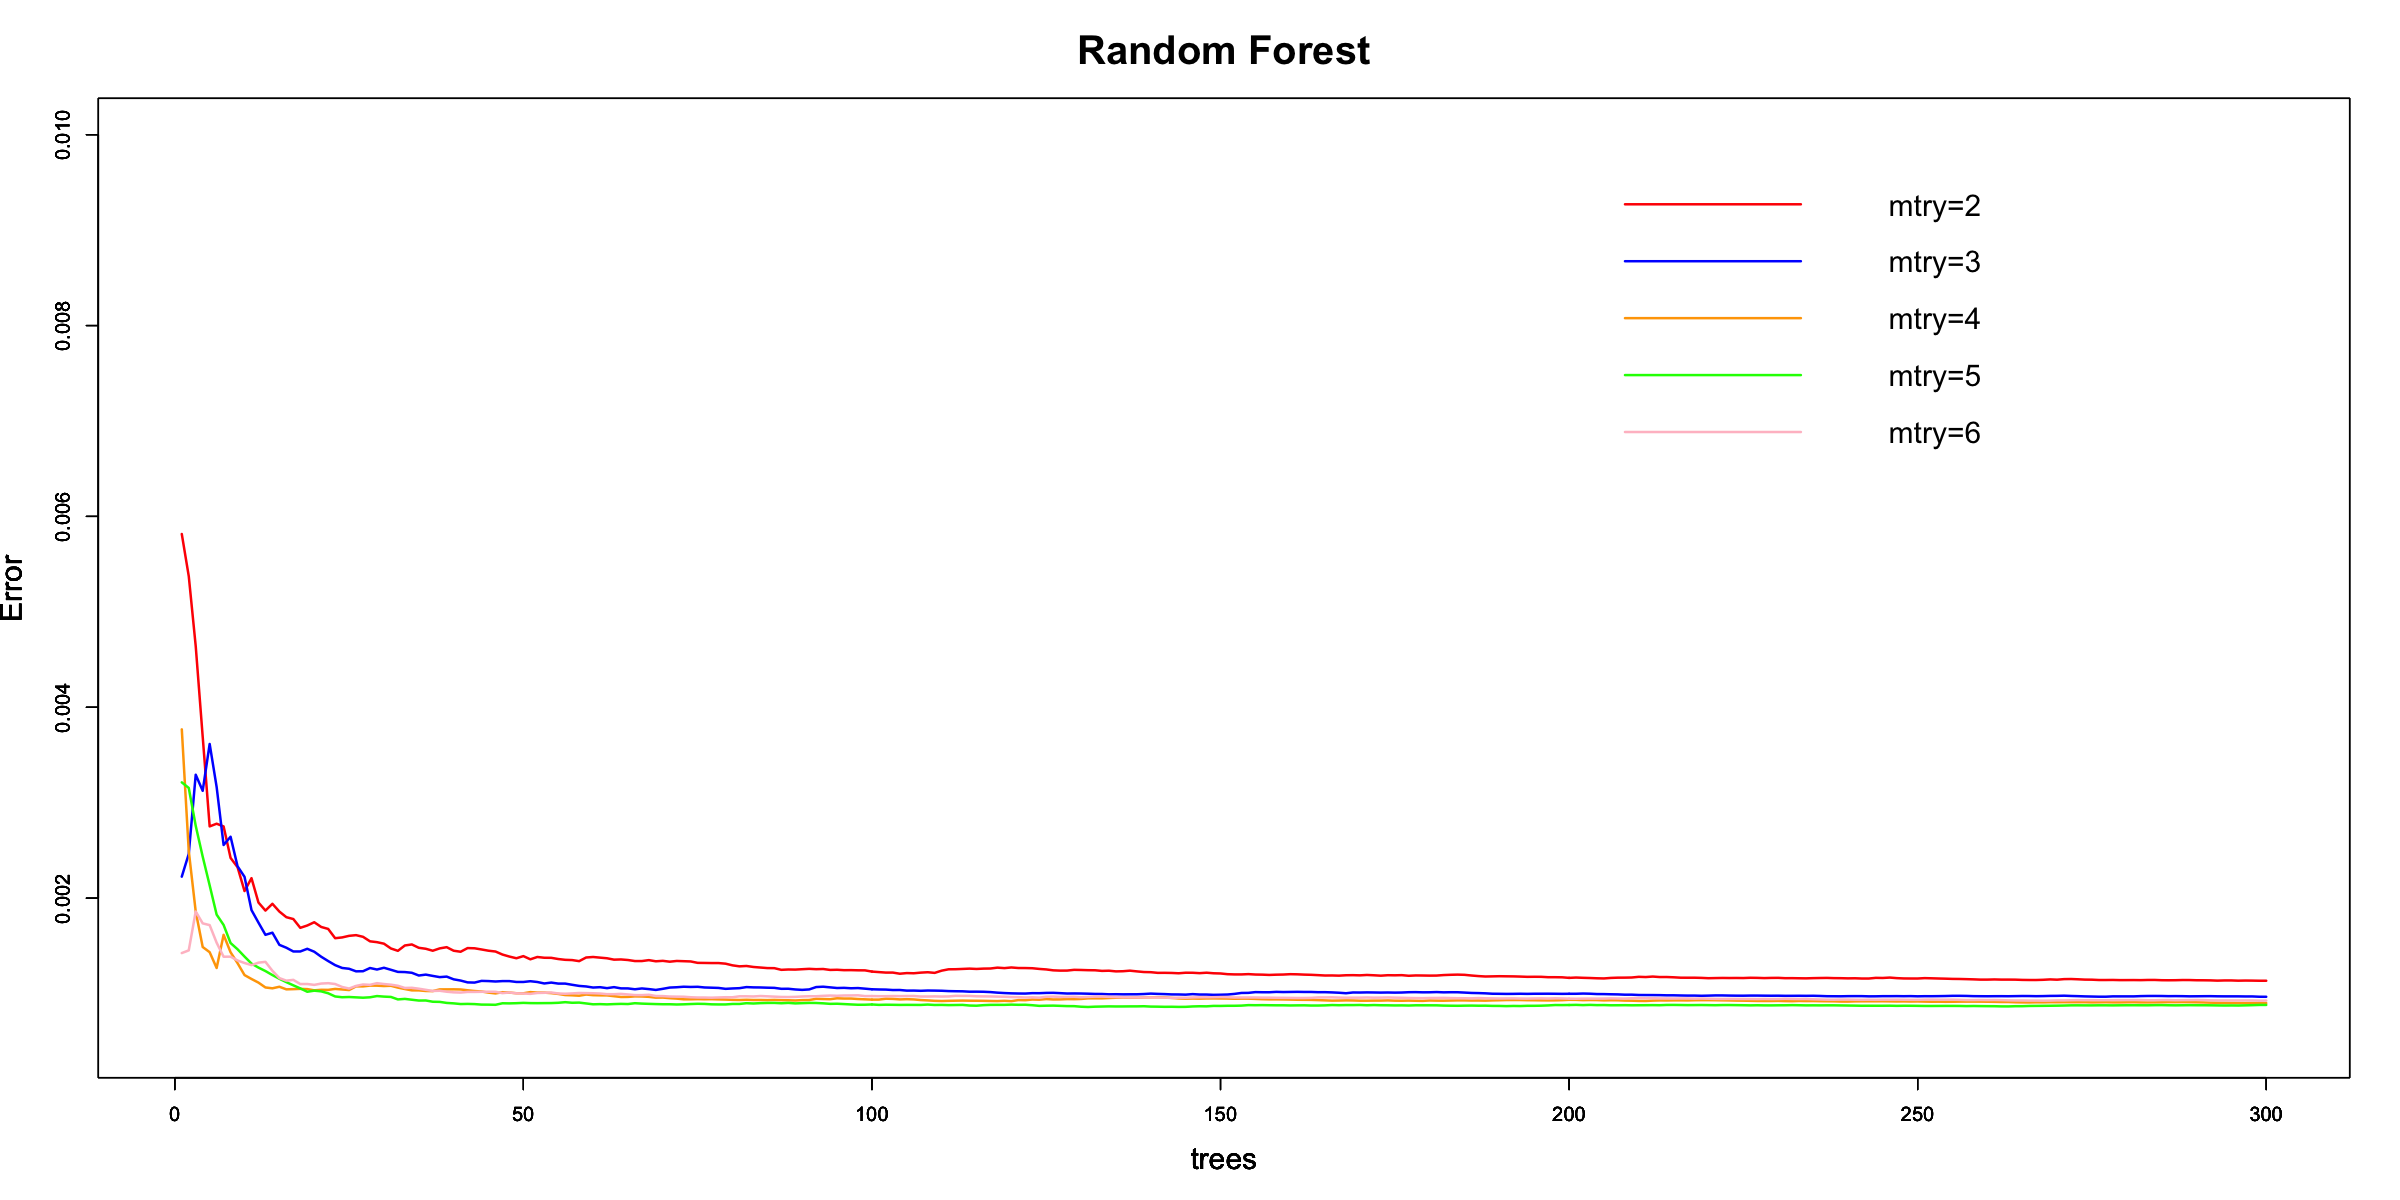
\includegraphics[width=7cm]{Figure/4.2.4-RF-200TreesStable.png}
  \end{subfigure}
  \begin{subfigure}{7.5cm}
    \centering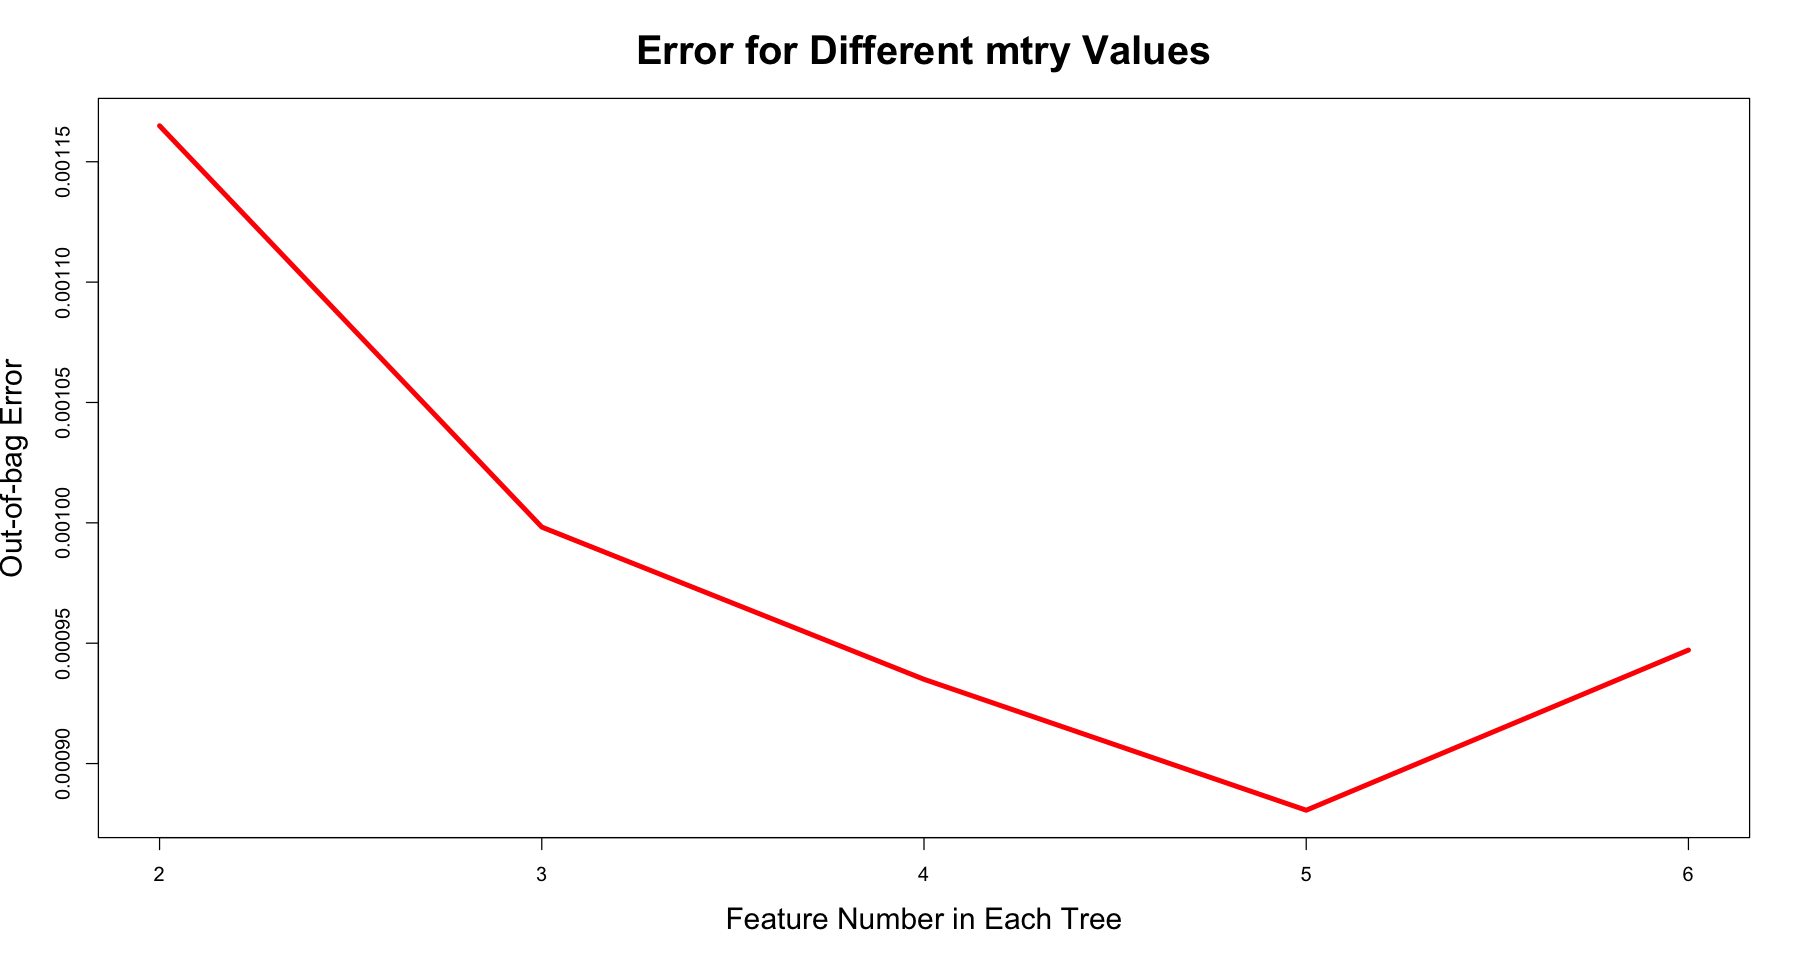
\includegraphics[width=7cm]{Figure/4.2.4-RF-5Features.png}
  \end{subfigure}
  \caption{Left: Check the error stability of random forest with different number of trees. Right: Check the out-of-bag error of random forest with different number of features in each tree when three number is 200.}
  \label{4.2.6-RF-200Trees-5Features}
\end{figure}

Moreover, the choice of the \sys{mtry} value is also important. Based on the selected tree number, different out-of-bag errors would be obtained by using different \sys{mtry} values. Through comparison, feature number in each tree was selected as 5 which corresponds with the minimum out-of-bag error.

After parameter was selected, Random Forest model was trained and tested. The MSE value is 0.00105 which is much smaller than the previous models. Observing the fitting diagram (bottom of Figure \ref{4.2.6-RFMSE}), it was found that dots were distributed in a narrow area fitting the straight line $y=x$, which indicates a robust fitting performance.

\begin{figure}[htbp]
\centering
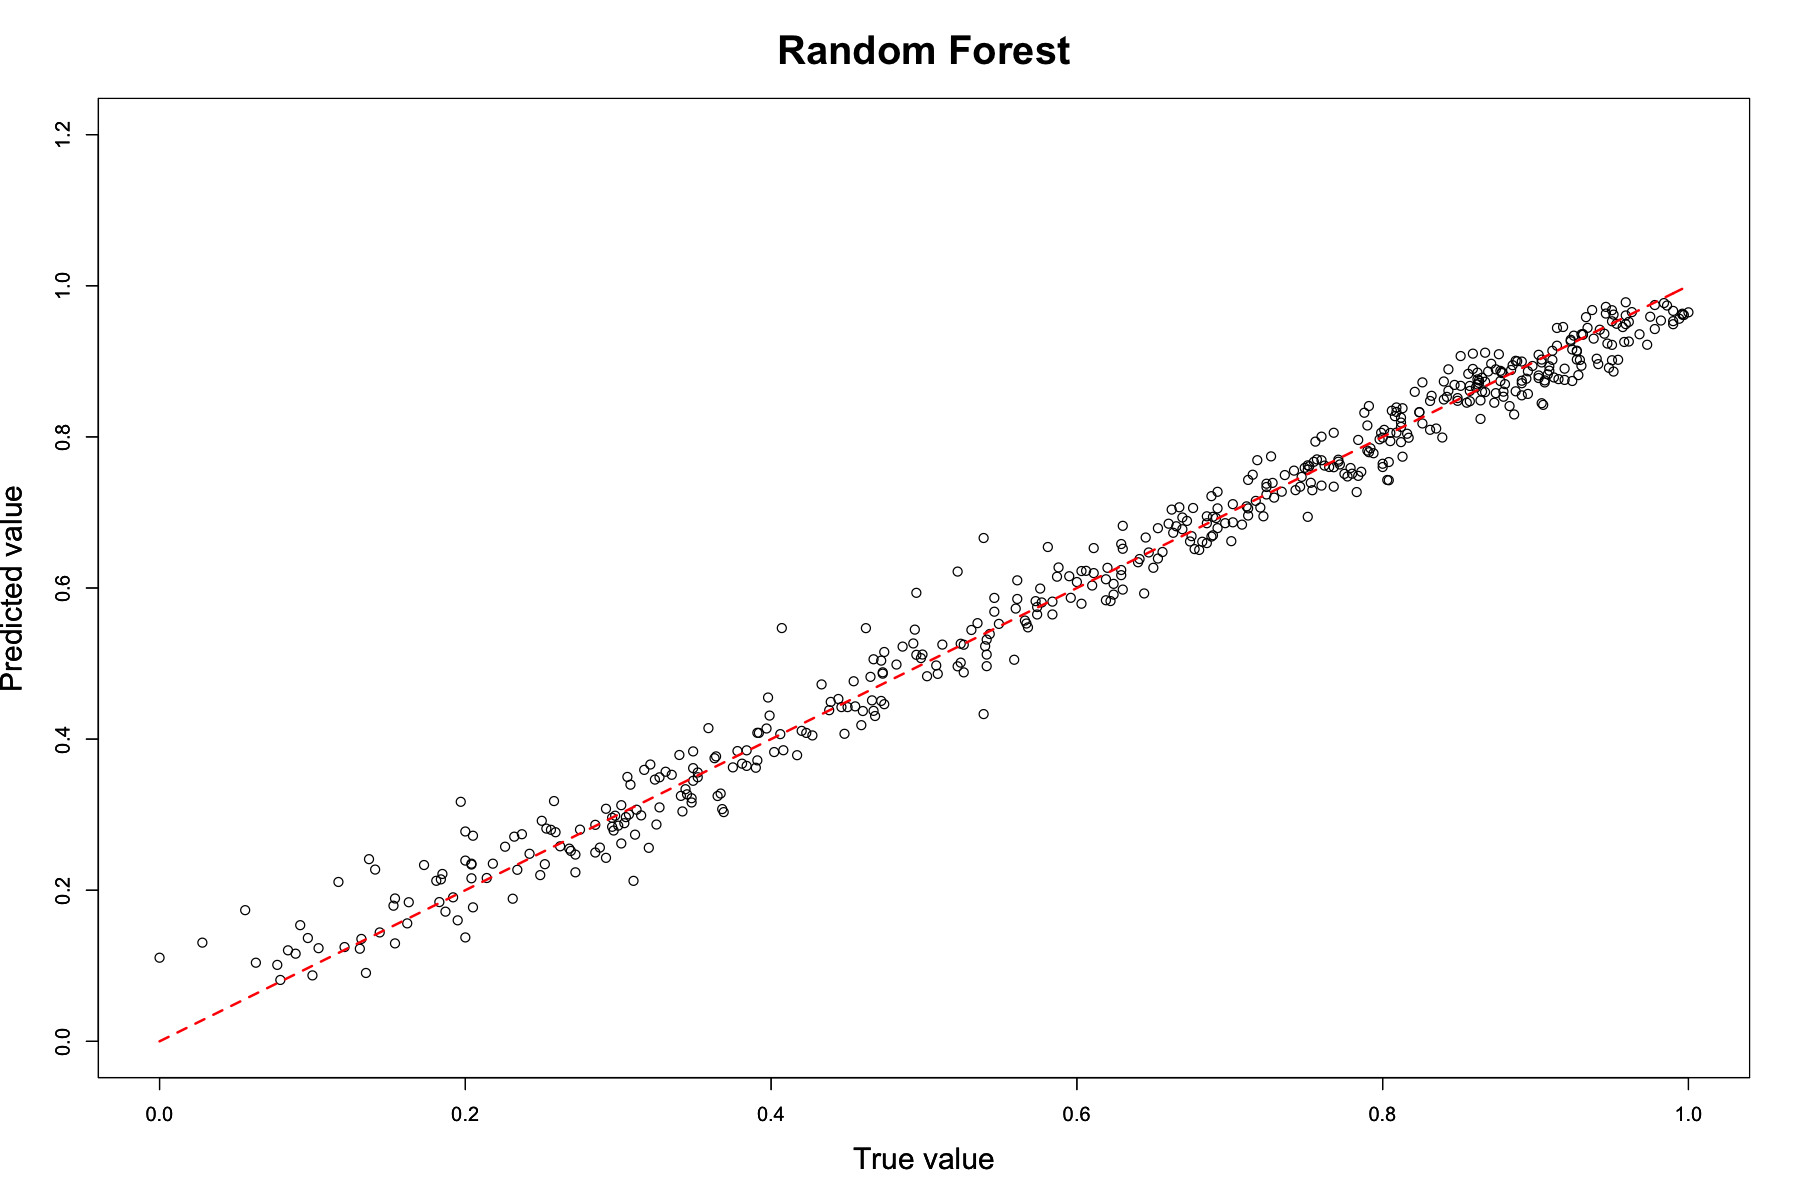
\includegraphics[width = 1.0\textwidth]{Figure/4.2.4-RF.png}
\caption{The predicted Arctic sea ice extent value vs the real Arctic sea ice extent value with \textbf{Random Forest} (200 trees, 5 features). The red referenced dotted line represents the straight line y=x. Mean Square Error (MSE) is \textbf{0.00105}.}
\label{4.2.6-RFMSE}
\end{figure}



\newpage
\section{Neural Network} %4.6

Unlike random forests, parameters are selected based on out-of-pocket errors in Neural Networks (NN). During the parameter tuning process, k-fold was applied on output testing errors for reference. After multiple tuning, 5 hidden layers were selected. Nine, seven, five, three and one neurons were used in each hidden layer from front to back as Figure \ref{4.2.5-NN-Structure} shown.

\begin{figure}[htbp]
\centering
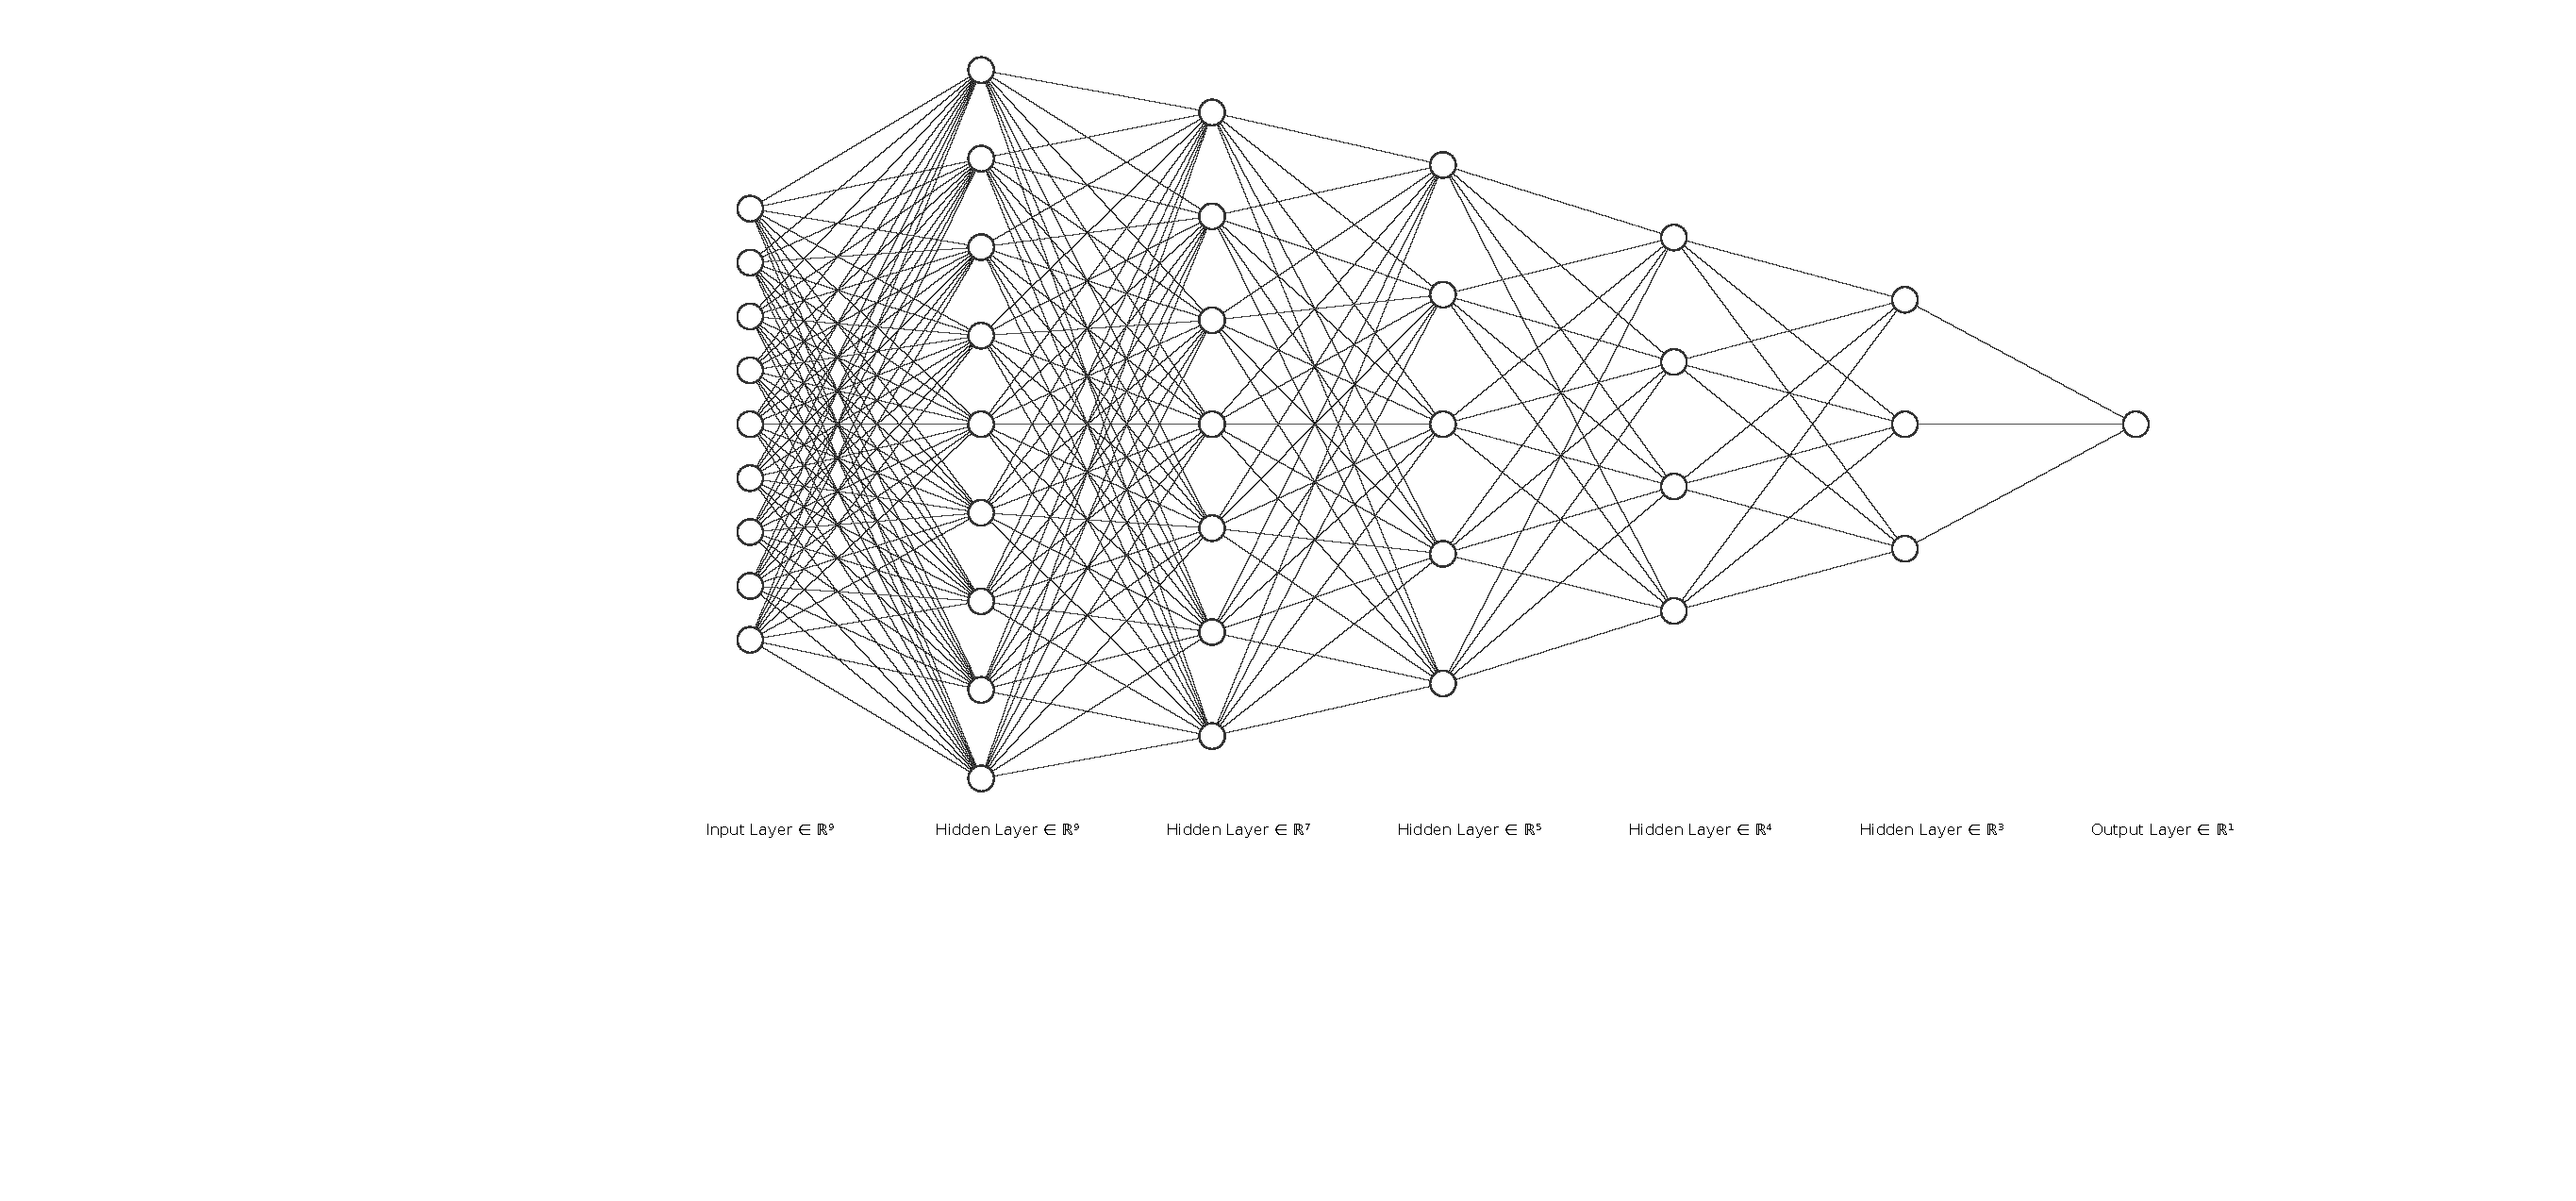
\includegraphics[width = 1.0\textwidth]{Figure/4.2.5-NN-Structure.pdf}
\caption{Neural Networks Structure.}
\label{4.2.5-NN-Structure}
\end{figure}


Similar to Random Forest, the Neural Network algorithm achieved excellent performance. The MSE value of Neural Network was slightly higher than the Random Forest, reaching 0.00106. The fitting diagram (right of Figure \ref{4.2.5-NN}) also proves that the variance of the Neural Networks model is very low comparing with previous Supervised Learning algorithms excluding Random Forest.


\begin{figure}[htbp]
\centering
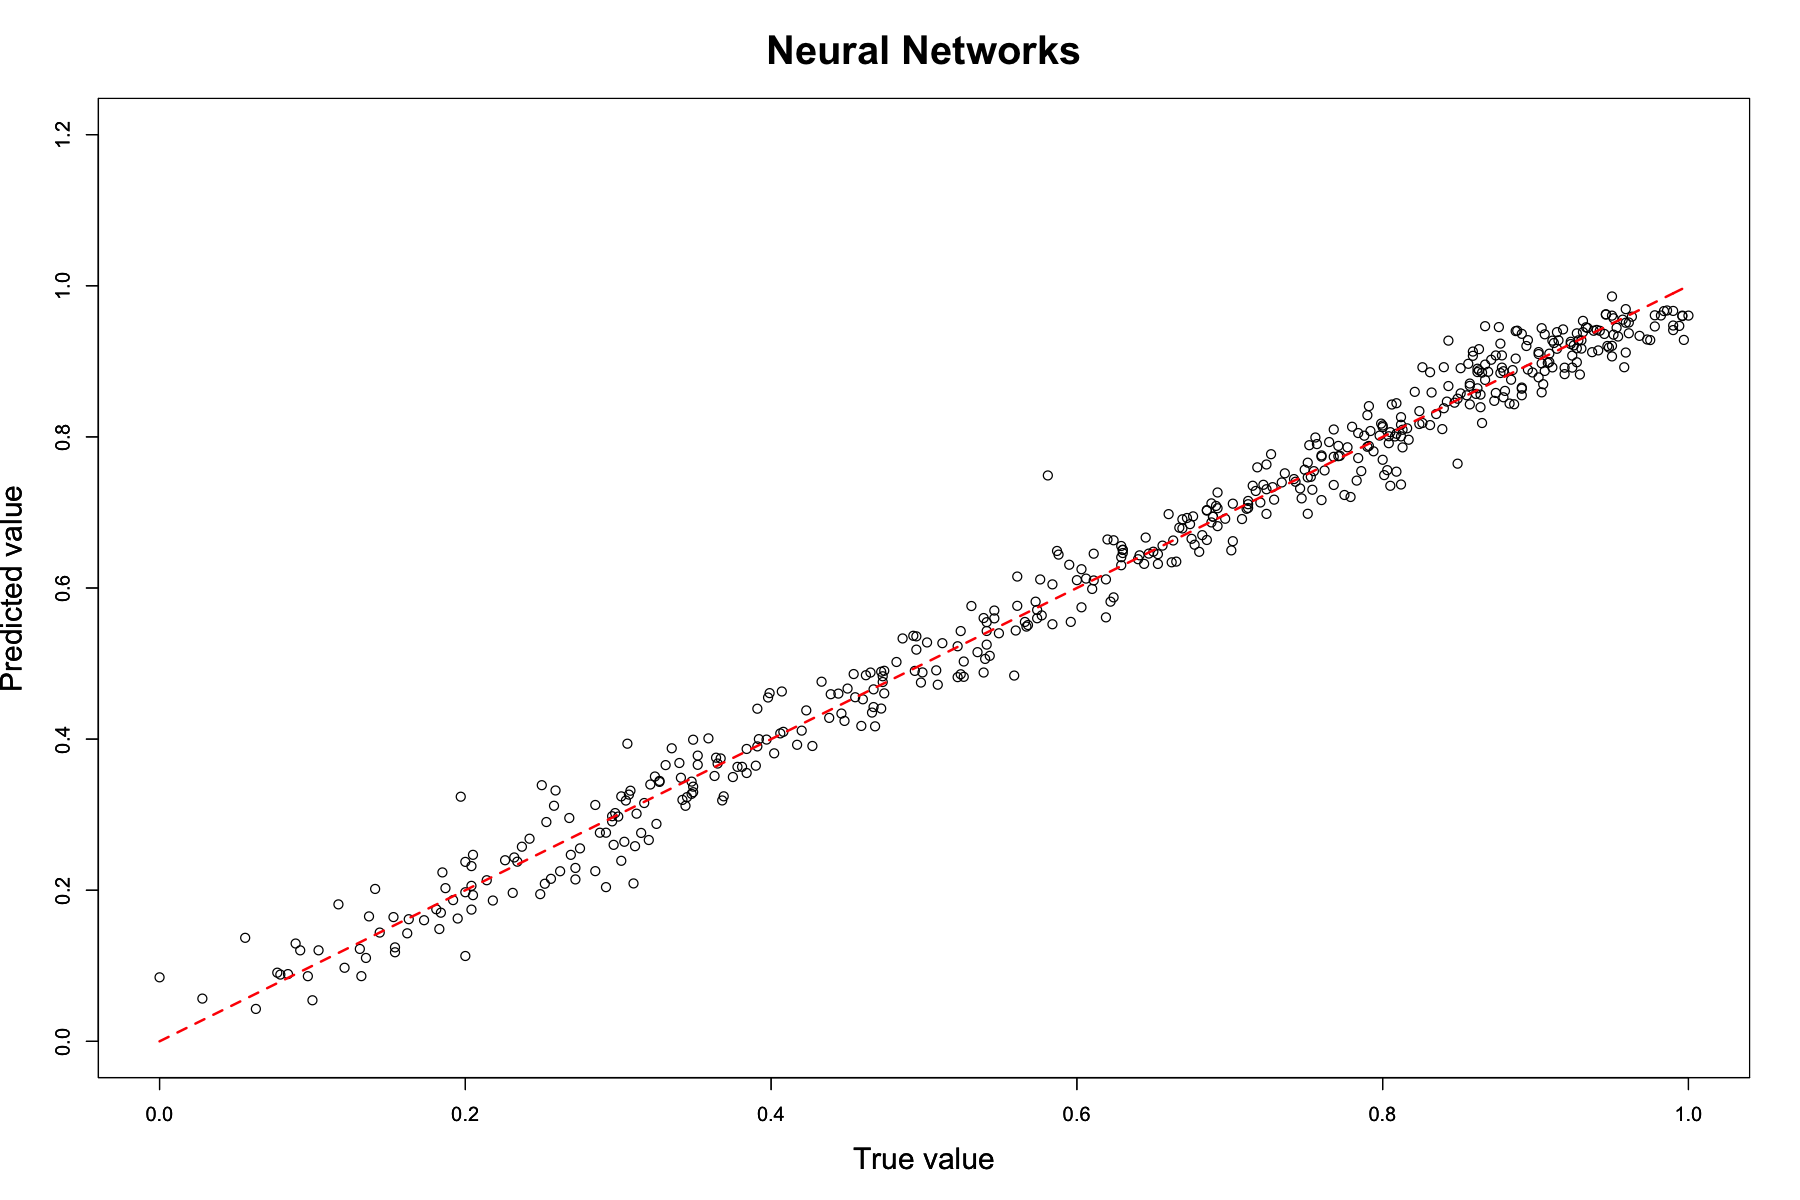
\includegraphics[width = 1.0\textwidth]{Figure/4.2.5-NN.png}
\caption{The predicted Arctic sea ice extent value vs the real Arctic sea ice extent value with \textbf{Neural Networks} (9 neurons, 5 hidden layers with (9,7,5,4,3) nodes respectively). The red referenced dotted line represents the straight line y=x. Mean Square Error (MSE) is \textbf{0.00106}.}
\label{4.2.5-NN}
\end{figure}


\newpage
\section{Comparison} %4.7
\label{sec:Comparison}
Based on the above four models and seven prediction results, all the results of R-squared and MSE are listed and compared in Table \ref{4.2.6-TABLE}. 

\begin{table}[htbp]
  \centering
  \footnotesize
  \begin{tabular}{p{6.7cm} | c | c}
  \toprule
  Model & $\text{R}^2$ & MSE\\ %row 1
  \hline
  Linear Regression & 0.898 & 0.00946\\
  Penalized Linear Regression (Lasso, min) & 0.863 & 0.00690\\
  Penalized Linear Regression (Lasso, 1se) & 0.857 & 0.00734\\
  Penalized Polynomial Regression (Lasso, min) & 0.931 & 0.00448\\
  Penalized Polynomial Regression (Lasso, 1se) & 0.917 & 0.00483\\
  Random Forest & \textbf{0.983} & \textbf{0.00105}\\
  Neural Networks & 0.927 & 0.00106\\
  \bottomrule
  \end{tabular}
  \caption{Comparison of performance metrics.}
  \label{4.2.6-TABLE}
\end{table}

Random Forest was selected for further future predictions as it was the best-performed model. As we can see from Table \ref{4.2.6-TABLE}, the model with low $\text{R}^2$ might not perform well, which indirectly proves the existence of over-fitting phenomenon and the necessity of penalization as well.


\chapter{Future Forecasting Results}   % Chapter 5
\label{Chapter5:Future-Results}
% section:
\section{Normal Situation} %5.1

Applying data sets which contains features for prediction (mentioned in Section \ref{sec:normal-predic}), the Arctic Sea Ice Extent variation in 10 years (from 2021 to 2030) was plotted (Figure \ref{4.3.1-10yrs}).

\begin{figure}[htbp]
\centering
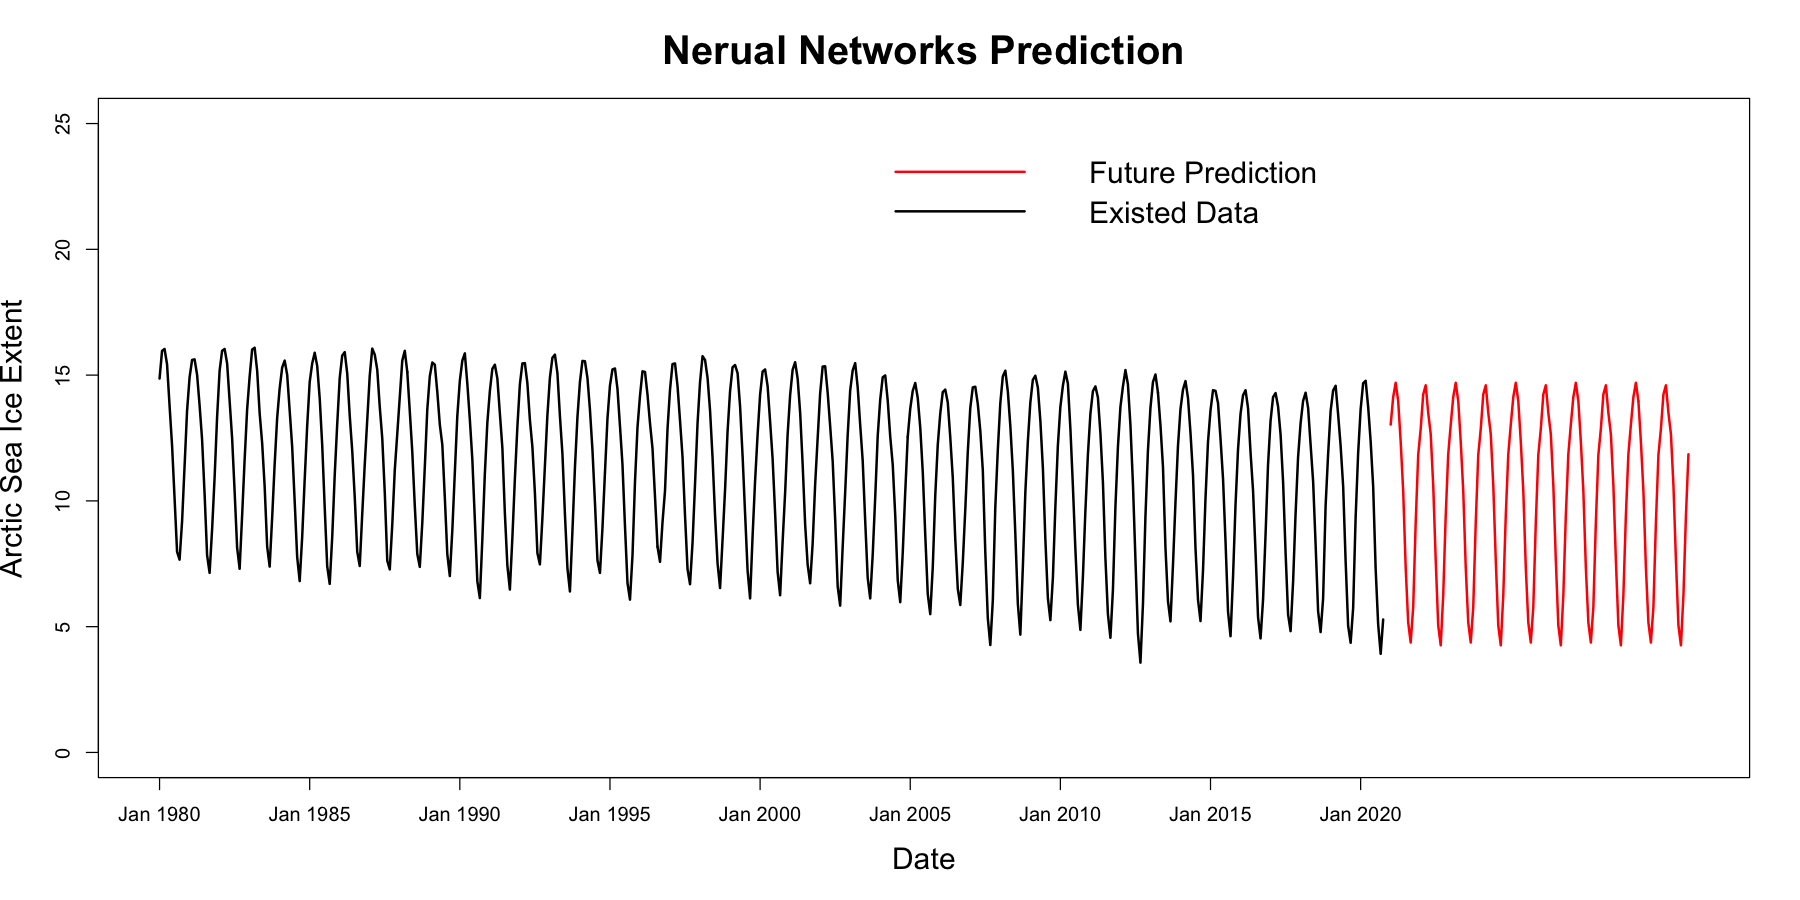
\includegraphics[width = 1.0\textwidth]{Figure/4.3.1-10yrs.png}
\caption{Future prediction of Arctic sea ice: 10 years' normal situation prediction ---- monthly.}
\label{4.3.1-10yrs}
\end{figure}


As the monthly figure (Figure \ref{4.3.1-Normal-Prediction}) shown, the sea ice extent fluctuation conforms to the expected seasonality and continues the main trend. Therefore, we can conclude that the prediction based on the neural network and the prediction data set is reasonable.

\begin{figure}[htbp]
\centering
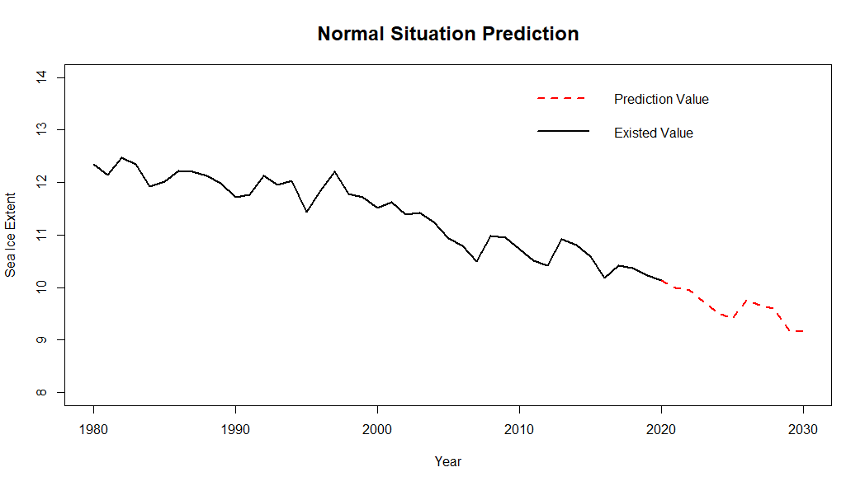
\includegraphics[width = 1.0\textwidth]{Figure/4.3.1-Normal-Prediction.png}
\caption{Future prediction of Arctic sea ice: 50 years' normal situation prediction.}
\label{4.3.1-Normal-Prediction}
\end{figure}

To predict a long-term trend, it is more intuitive to visualize using annual average. Based on Random Forest model, the Arctic sea ice extent decreased from 10.00 $\text{Mkm}^2$ in 2020 to 9.41 $\text{Mkm}^2$ in 2030, reducing by 5.9\%.

\newpage
\section{Special Situation} %5.2
First, visualizations were performed using \sys{Variable Importance} function. According to Figure \ref{4.3.2-Variance-Importance}, it can be seen that ozone, rainfall, and temperature are the most important features. However, rainfall is not as closely related to climate change as temperature, so we chose ozone and temperature as two key factors.

\begin{figure}[htbp]
\centering
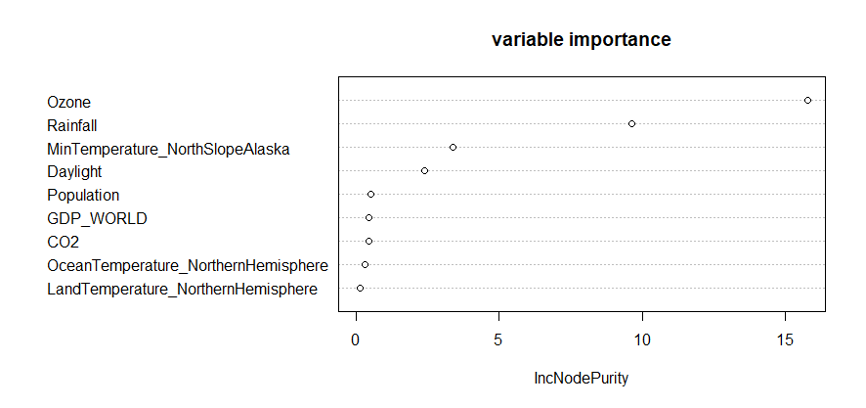
\includegraphics[width = 1.0\textwidth]{Figure/4.3.2-Variance-Importance.png}
\caption{Comparison of variance importance.}
\label{4.3.2-Variance-Importance}
\end{figure}

Linear Regression was applied on annul average ozone value only, a straight line was plotted and the ozone level decreased by 4.6\% in last 40 years. Based on the \sys{Normal Situation} data processing (Section \ref{sec:normal-predic}), the ozone level was predicted to decrease about 1.2\% in 10 years. For generating ozone data of \sys{Special Situation}, a ramp was applied on \sys{Normal Situation} data for simulating ozone variation in high level where it was decreased by 2.5\% in 10 years and low level where it was set no variation in 10 years).

\begin{figure}[htbp]
\centering
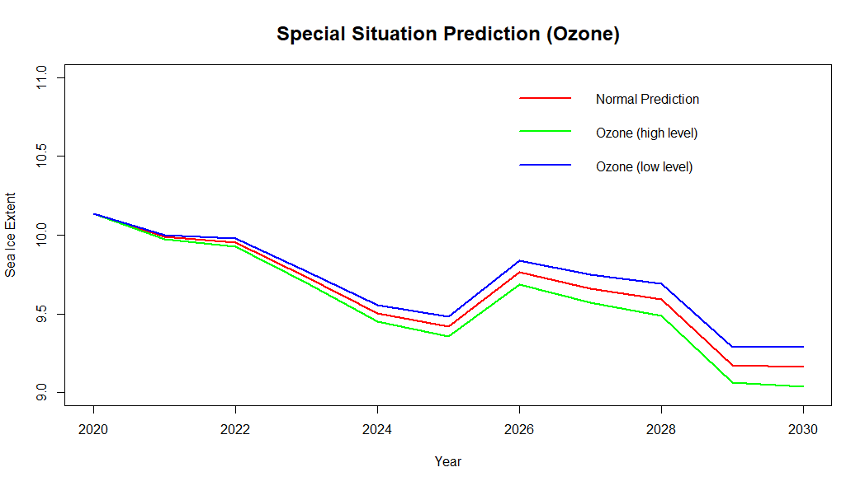
\includegraphics[width = 1.0\textwidth]{Figure/4.3.2-Emergency-Prediction-Ozone.png}
\caption{Special situation prediction based on different Ozone level.}
\label{4.3.2-Emergency-Prediction-Ozone}
\end{figure}

As Figure \ref{4.3.2-Emergency-Prediction-Ozone} shown, applying high level ozone, the predicted extent of Arctic sea ice was 0.92\% lower than applying Normal Situation, which was 9.414 $\text{Mkm}^2$. Moreover, applying low level ozone level, the predicted result was 0.87\% higher than that of \sys{Normal situation}. There was a negative correlation between ozone level and Arctic ice extent, which further confirmed the relationship shown in correlation matrix.

Similarly, applying the same method on \textit{MinTemperature}, in high level, normal situation and low level, the temperature was set to rise by 7,4,1 degree Celsius respectively.


\begin{figure}[htbp]
\centering
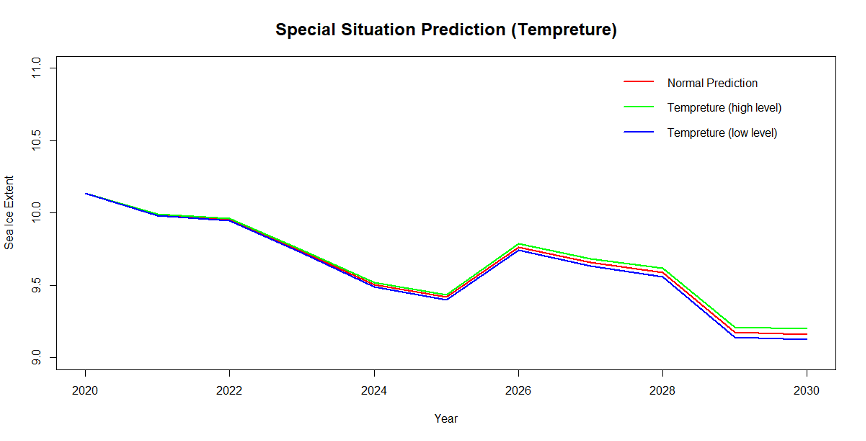
\includegraphics[width = 1.0\textwidth]{Figure/4.3.2-Emergency-Prediction-Temp.png}
\caption{Special situation prediction based on different minimum temperature level in North Slope Alaska.}
\label{4.3.2-Emergency-Prediction-Temp}
\end{figure}

According to the results above (Figure \ref{4.3.2-Emergency-Prediction-Temp}), applying high level temperature, the predicted extent of Arctic sea ice was 0.13\% higher than applying Normal Situation. While applying low level ozone level, the predicted result was 0.16\% lower than \sys{Normal situation}. It was found that the temperature is positively correlated with the Arctic sea ice extent from the correlation matrix. In addition, the influence of temperature change on the sea ice extent is not as sensitive as ozone, which also proved the feature importance of temperature is lower than ozone.


\chapter{Conclusion}                            % Chapter 6
\label{Chapter6:Conclusion}
% section:
% Chapter 5: Conclusion






% Bibliography
\bibliographystyle{IEEEtran}
\bibliography{ref}

\end{document}